% =========================================================================
% PROTOCOLO EXPERIMENTAL E BENCHMARKS COMPUTACIONAIS
% =========================================================================
\chapter{Protocolo Experimental e Benchmarks Computacionais}\label{sec:benchmarks}

Para avaliar o desempenho prático dos algoritmos em relação às suas garantias assintóticas teóricas, estruturamos uma bateria de testes experimentais documentada em \code{experiments/}. Este capítulo detalha o protocolo metodológico, as instâncias de teste e os resultados comparativos obtidos.


\section{Rigor Metodológico e Ambiente de Teste}\label{sec:bench_metodologia}

Para assegurar rigor científico e reprodutibilidade, todos os experimentos foram executados em uma estação de trabalho com processador \textbf{Intel Core i5-13500} de 13ª geração (14 núcleos e 20 threads lógicos, até 4,8 GHz Turbo), 32 GB de memória RAM DDR4, sob o sistema operacional \textbf{Windows 11 Build 26H2} com ambiente POSIX \textbf{MSYS2 (UCRT64)} e arquitetura \texttt{x86\_64}.

O protocolo experimental fundamenta-se nas seguintes diretrizes:

\begin{enumerate}
    \item \textbf{Isolamento Estrito e Execução Paralela Concorrente:} O tempo de CPU é medido com \lstinline{std::chrono::steady_clock} (C++23), cronometrando individualmente a execução de cada motor de fluxo em instâncias independentes. Os algoritmos avaliados para cada instância são disparados concorrentemente em threads paralelas sobre os múltiplos núcleos do processador, garantindo eficiência de medição sem perda de isolamento analítico.
    \item \textbf{Parâmetros de Compilação e Otimização:} O código-fonte é compilado com GCC/Clang sob o padrão ISO C++23 com nível de otimização \lstinline{-O2}.
    \item \textbf{Tratamento Estatístico e Controle de Timeout:} Cada instância é executada de forma independente por $N = 2$ repetições em regime estacionário (\textit{steady state}), descartando o aquecimento de cache. Registram-se a média e o desvio-padrão. Fixa-se o limite de 16 segundos por instância.
\end{enumerate}


\section{Famílias de Instâncias Padronizadas da Literatura (DIMACS)}\label{sec:bench_instancias}

Para submeter os algoritmos a diferentes desafios estruturais de rede, a avaliação experimental adota 80 instâncias padronizadas de referência do \textit{First DIMACS International Algorithm Implementation Challenge} (1990--1991)~\cite{Jensen2022, ahuja1993network}, distribuídas simetricamente entre Fluxo Máximo e Fluxo de Custo Mínimo, acrescidas de uma suíte específica para Grafos Bipartidos:

\begin{itemize}
    \item \textbf{Família DIMACS Max-Flow (40 instâncias):}
    \begin{itemize}
        \item \textbf{Washington Mesh (8 instâncias):} Redes em malha bidimensional plana de dimensão progressiva ($16 \times 16$ a $128 \times 128$) com capacidades aleatórias, avaliando escalabilidade em grafos planares;
        \item \textbf{Washington RLG (8 instâncias):} Redes de camadas aleatórias (\textit{Random Level Graphs}) com conectividade direcionada por níveis;
        \item \textbf{Washington Line (6 instâncias):} Cadeias lineares longas com gargalos induzidos para provocar caminhos aumentantes de comprimento $\Omega(|V|)$;
        \item \textbf{Washington Exp-Line (4 instâncias):} Redes lineares com capacidades variando exponencialmente, projetadas para testar a dependência pseudo-polinomial em relação a $|f^*|$;
        \item \textbf{Washington Adversariais e Emparelhamento (4 instâncias):} Estruturas adversariais construídas especificamente para pior caso de Dinic (\texttt{bad\_dinic}) e de Goldberg (\texttt{bad\_gold}), além de emparelhamentos bipartidos densos (\texttt{wash\_match});
        \item \textbf{Genrmf (10 instâncias):} Grafos tridimensionais formados por planos bidimensionais interconectados com capacidades aleatórias (\textit{small}, \textit{medium}, \textit{wide}, \textit{long}, \textit{huge}, \textit{cube} e \textit{deep}), onde a fonte reside no primeiro plano e o sumidouro no último, impondo cortes mínimos estreitos.
    \end{itemize}

    \item \textbf{Família DIMACS Min-Cost Flow (40 instâncias):}
    \begin{itemize}
        \item \textbf{Netgen (Problemas 01 a 10):} Redes de transporte e transbordo esparsas ($|V| \approx 200 \dots 300$, $|A| \approx 1.500 \dots 6.600$) com oferta e demanda concentradas;
        \item \textbf{Netgen (Problemas 11 a 20):} Redes com capacidades amplas e fontes distribuídas ($|V| \approx 400 \dots 500$), avaliando a robustez de métodos de cancelamento de ciclos e caminhos mínimos sucessivos;
        \item \textbf{Netgen (Problemas 21 a 30):} Redes densas com custos uniformemente distribuídos ($|V| \approx 1.000$, $|A| \approx 3.000 \dots 9.000$);
        \item \textbf{Netgen (Problemas 31 a 40):} Instâncias de grande porte e casos limites da literatura ($|V| \approx 1.500 \dots 3.000$, $|A| \approx 4.000 \dots 35.000$).
    \end{itemize}

    \item \textbf{Suíte Bipartida de Emparelhamento e Atribuição (18 instâncias):}
    \begin{itemize}
        \item \textbf{Emparelhamento Bipartido (10 instâncias):} Grafos bipartidos esparsos (\texttt{bip\_sparse}), densos (\texttt{bip\_dense}), regulares (\texttt{bip\_regular}) e com longos caminhos alternantes (\texttt{bip\_trap}), comparando \lstinline{Kuhn} e \lstinline{HopcroftKarp} aos seis motores gerais de fluxo máximo;
        \item \textbf{Atribuição Bipartida Ponderada (8 instâncias):} Matrizes de atribuição com custos uniformes (\texttt{assign\_uniform}), custos de grande magnitude (\texttt{assign\_highcost}) e distâncias euclidianas (\texttt{assign\_euclid}), comparando \lstinline{KuhnMunkres} aos quatro motores gerais de custo mínimo.
    \end{itemize}
\end{itemize}


\section{Métricas Operacionais e Certificação Cruzada de Corretude}\label{sec:bench_metricas}

Além do tempo de execução, a instrumentação computacional coleta métricas que refletem a dinâmica de cada algoritmo:

\begin{enumerate}
    \item \textbf{Contadores de Fases e Operações Elementares:}
    \begin{itemize}
        \item Em Ford-Fulkerson e Edmonds-Karp, quantificam-se a quantidade de caminhos aumentantes e o comprimento médio desses caminhos;
        \item No algoritmo de Dinic, contabilizam-se as fases de construção do digrafo de níveis e a quantidade de avanços e retrocessos de ponteiro na DFS de fluxo bloqueador;
        \item Na família Push-Relabel, monitoram-se separadamente as operações de empurrão (\textit{pushes}, saturantes e não saturantes) e de elevação (\textit{relabels}), evidenciando a eliminação de vértices desconectados do sumidouro pela heurística de lacuna (\textit{Gap Heuristic});
        \item No algoritmo \textit{Network Simplex}, registram-se o total de pivoteamentos de base e a proporção de pivôs degenerados (onde o fluxo do arco entrante é zero).
    \end{itemize}

    \item \textbf{Verificação Automática da Otimalidade e Consistência (Validação Cruzada):} O programa de testes verifica se todos os algoritmos produzem o mesmo valor ótimo:
    \begin{gather}
        |f^*_{\text{Edmonds-Karp}}| = |f^*_{\text{Dinic}}| = |f^*_{\text{Push-Relabel}}|, \\
        z^*_{\text{CycleCanceling}} = z^*_{\text{MMCC}} = z^*_{\text{CancelAndTighten}} = z^*_{\text{SSP}} = z^*_{\text{NetworkSimplex}}
    \end{gather}
    Essa checagem cruzada previne discrepâncias de implementação ou instabilidades numéricas.
\end{enumerate}


\section{Quadro-Molde de Comparação dos Motores Algorítmicos}

A Tabela~\ref{tab:benchmarks} sintetiza o comportamento operacional esperado de cada algoritmo frente às diferentes famílias de redes.

\begin{table}[!ht]
\centering
\small
\setlength{\tabcolsep}{4.5pt}
\begin{tabular}{p{3.6cm} p{5.4cm} p{5.7cm}}
\toprule
\multicolumn{1}{c}{\textbf{Motor Algorítmico (C++)}} & \multicolumn{1}{c}{\textbf{Família de Melhor Desempenho}} & \multicolumn{1}{c}{\textbf{Cenário Crítico e Gargalo Empírico}} \\
\midrule
\multicolumn{3}{c}{\bannertext{\hyperref[sec:bench_instancias]{Motores de Fluxo Máximo (Coleções DIMACS Washington e RMF)}}} \\
\midrule
\hyperref[ap:ford_fulkerson]{Ford-Fulkerson} & Capacidades pequenas e caminhos curtos & Capacidades exponenciais e redes com ciclos \\
\hyperref[ap:edmonds_karp]{Edmonds-Karp} & Redes esparsas com poucos aumentos globais & Redes em camadas profundas (custo de BFSs sucessivas) \\
\hyperref[ap:dinic]{Dinic} & Redes unitárias, grafos bipartidos e redes densas & Gargalos múltiplos em níveis sucessivos da rede \\
\hyperref[ap:mpm]{MPM} & Digrafos em níveis densos com grau elevado & Varredura de potenciais nodais $\mathcal{O}(|V|^2)$ em grafos muito esparsos \\
\hyperref[ap:push_relabel]{Push-Relabel (FIFO)} & Redes densas com cortes mínimos próximos à fonte & Cadeias longas sem saturação imediata de excessos \\
\hyperref[ap:push_relabel_improved]{Push-Relabel (Gap)} & Grafos de visão (grid 2D/3D) e instâncias DIMACS RMF & Gargalos com desconexões sucessivas do sumidouro (eliminadas por Gap) \\
\hyperref[ap:kuhn]{Kuhn} / \hyperref[ap:hopcroft_karp]{Hopcroft-Karp} & Emparelhamento bipartido unitário ($s \to L \to R \to t$) & Restritos a redes bipartidas unitárias (fallback residual nos demais casos) \\
\midrule
\multicolumn{3}{c}{\bannertext{\hyperref[sec:bench_instancias]{Motores de Fluxo de Custo Mínimo (Coleção DIMACS Netgen)}}} \\
\midrule
\hyperref[ap:cycle_canceling]{Cycle Canceling} & Redes pequenas com poucos ciclos de custo negativo & Custos residuais elevados com múltiplos ciclos de $-1$ \\
\hyperref[ap:minimum_mean_cycle_canceling]{Minimum-Mean CC} & Redes esparsas de pequeno porte e fluxo nulo & Recálculo de Karp $\mathcal{O}(|V||A|)$ a cada fase em instâncias com $|V| \ge 1.500$ \\
\hyperref[ap:cancel_and_tighten]{Cancel-and-Tighten} & Redes médias e densas com múltiplos ciclos negativos & Redes esparsas de grande porte ($|V| \ge 5.000$) sob limite de 16 s \\
\hyperref[ap:successive_shortest_dijkstra]{SSP (Dijkstra + $\pi$)} & Redes de transbordo com fluxo total moderado & Redes com fluxos massivos e capacidades unitárias \\
\hyperref[ap:network_simplex]{Network Simplex} & Grafos em grade, instâncias Netgen e redes logísticas & Degenerescência cíclica severa (controlada por Cunningham) \\
\hyperref[ap:kuhn_munkres]{Kuhn-Munkres (Húngaro)} & Atribuição bipartida densa ($|L| = |R|$) & Matrizes densas $\mathcal{O}(|V|^3)$ frente a grafos muito esparsos \\
\bottomrule\end{tabular}
\caption{Quadro de análise comparativa dos motores algorítmicos e sensibilidade estrutural frente aos conjuntos de teste.}
\label{tab:benchmarks}
\end{table}

Os scripts no diretório \code{experiments/} automatizam a execução deste protocolo e geram as tabelas e gráficos apresentados a seguir.


\section{Resultados Experimentais: Fluxo Máximo}\label{sec:bench_resultados_maxflow}

A Tabela~\ref{tab:results_maxflow} apresenta os tempos médios de execução ($\bar{t}$ em ms) e o fluxo ótimo $f^*$ obtidos pelos seis algoritmos de fluxo máximo (\lstinline{FordFulkerson}, \lstinline{EdmondsKarp}, \lstinline{Dinic}, \lstinline{MPM}, \lstinline{PushRelabel} e \lstinline{PushRelabelImproved}) nas 40 instâncias de referência DIMACS (Washington e Genrmf). O menor tempo por instância está destacado em \textbf{negrito}.

\IfFileExists{book/tables/table_max_flow.tex}{
\begingroup
\small
\setlength{\tabcolsep}{4pt}
\begin{longtable}{llrrrrl}
\caption{Resultados experimentais dos motores de fluxo máximo.}\label{tab:results_maxflow}\\
\toprule
\textbf{Instância} & \textbf{Algoritmo} & $|V|$ & $|A|$ & $f^*$ & $\bar{t}$ (ms) & \textbf{Status} \\
\midrule
\endfirsthead
\caption[]{Resultados experimentais dos motores de fluxo máximo (continuação)}\\
\toprule
\textbf{Instância} & \textbf{Algoritmo} & $|V|$ & $|A|$ & $f^*$ & $\bar{t}$ (ms) & \textbf{Status} \\
\midrule
\endhead
\bottomrule
\endfoot
genrmf\_cube\_10.max & Dinic & 1000 & 4500 & 201007 & 1.77 & OK \\
genrmf\_cube\_10.max & PushRelabelImproved & 1000 & 4500 & 201007 & \textbf{1.33} & OK \\
genrmf\_cube\_10.max & PushRelabel & 1000 & 4500 & 201007 & 1.40 & OK \\
genrmf\_cube\_10.max & EdmondsKarp & 1000 & 4500 & 201007 & 4.37 & OK \\
genrmf\_cube\_10.max & FordFulkerson & 1000 & 4500 & 201007 & 5136.85 & OK \\
genrmf\_cube\_10.max & MPM & 1000 & 4500 & 201007 & 3.06 & OK \\
\midrule
genrmf\_cube\_16.max & Dinic & 4096 & 19200 & 519782 & 10.15 & OK \\
genrmf\_cube\_16.max & PushRelabelImproved & 4096 & 19200 & 519782 & 8.27 & OK \\
genrmf\_cube\_16.max & PushRelabel & 4096 & 19200 & 519782 & \textbf{8.19} & OK \\
genrmf\_cube\_16.max & EdmondsKarp & 4096 & 19200 & 519782 & 71.65 & OK \\
genrmf\_cube\_16.max & FordFulkerson & 4096 & 19200 & -1 & --- & TLE \\
genrmf\_cube\_16.max & MPM & 4096 & 19200 & 519782 & 22.47 & OK \\
\midrule
genrmf\_deep\_32.max & Dinic & 1152 & 4956 & 74207 & \textbf{1.49} & OK \\
genrmf\_deep\_32.max & PushRelabelImproved & 1152 & 4956 & 74207 & 1.72 & OK \\
genrmf\_deep\_32.max & PushRelabel & 1152 & 4956 & 74207 & 73.03 & OK \\
genrmf\_deep\_32.max & EdmondsKarp & 1152 & 4956 & 74207 & 3.68 & OK \\
genrmf\_deep\_32.max & FordFulkerson & 1152 & 4956 & 74207 & 1707.32 & OK \\
genrmf\_deep\_32.max & MPM & 1152 & 4956 & 74207 & 2.98 & OK \\
\midrule
genrmf\_deep\_64.max & Dinic & 2304 & 9948 & 74476 & \textbf{3.14} & OK \\
genrmf\_deep\_64.max & PushRelabelImproved & 2304 & 9948 & 74476 & 4.20 & OK \\
genrmf\_deep\_64.max & PushRelabel & 2304 & 9948 & 74476 & 5.01 & OK \\
genrmf\_deep\_64.max & EdmondsKarp & 2304 & 9948 & 74476 & 13.29 & OK \\
genrmf\_deep\_64.max & FordFulkerson & 2304 & 9948 & 74476 & 3609.49 & OK \\
genrmf\_deep\_64.max & MPM & 2304 & 9948 & 74476 & 8.21 & OK \\
\midrule
genrmf\_huge.max & Dinic & 4096 & 18368 & 129102 & \textbf{7.36} & OK \\
genrmf\_huge.max & PushRelabelImproved & 4096 & 18368 & 129102 & 14.04 & OK \\
genrmf\_huge.max & PushRelabel & 4096 & 18368 & 129102 & 1103.00 & OK \\
genrmf\_huge.max & EdmondsKarp & 4096 & 18368 & 129102 & 40.86 & OK \\
genrmf\_huge.max & FordFulkerson & 4096 & 18368 & -1 & --- & TLE \\
genrmf\_huge.max & MPM & 4096 & 18368 & 129102 & 20.07 & OK \\
\midrule
genrmf\_long.max & Dinic & 1024 & 4080 & 35848 & \textbf{1.33} & OK \\
genrmf\_long.max & PushRelabelImproved & 1024 & 4080 & 35848 & 1.58 & OK \\
genrmf\_long.max & PushRelabel & 1024 & 4080 & 35848 & 2.17 & OK \\
genrmf\_long.max & EdmondsKarp & 1024 & 4080 & 35848 & 3.11 & OK \\
genrmf\_long.max & FordFulkerson & 1024 & 4080 & 35848 & 580.20 & OK \\
genrmf\_long.max & MPM & 1024 & 4080 & 35848 & 2.80 & OK \\
\midrule
genrmf\_medium.max & Dinic & 1024 & 4544 & 132414 & 1.46 & OK \\
genrmf\_medium.max & PushRelabelImproved & 1024 & 4544 & 132414 & \textbf{1.33} & OK \\
genrmf\_medium.max & PushRelabel & 1024 & 4544 & 132414 & 60.37 & OK \\
genrmf\_medium.max & EdmondsKarp & 1024 & 4544 & 132414 & 3.45 & OK \\
genrmf\_medium.max & FordFulkerson & 1024 & 4544 & 132414 & 2807.06 & OK \\
genrmf\_medium.max & MPM & 1024 & 4544 & 132414 & 2.91 & OK \\
\midrule
genrmf\_small.max & Dinic & 256 & 1008 & 34555 & \textbf{0.26} & OK \\
genrmf\_small.max & PushRelabelImproved & 256 & 1008 & 34555 & 0.27 & OK \\
genrmf\_small.max & PushRelabel & 256 & 1008 & 34555 & 3.72 & OK \\
genrmf\_small.max & EdmondsKarp & 256 & 1008 & 34555 & 0.33 & OK \\
genrmf\_small.max & FordFulkerson & 256 & 1008 & 34555 & 69.67 & OK \\
genrmf\_small.max & MPM & 256 & 1008 & 34555 & 0.51 & OK \\
\midrule
genrmf\_wide.max & Dinic & 1024 & 4608 & 515228 & 2.50 & OK \\
genrmf\_wide.max & PushRelabelImproved & 1024 & 4608 & 515228 & \textbf{1.89} & OK \\
genrmf\_wide.max & PushRelabel & 1024 & 4608 & 515228 & 63.70 & OK \\
genrmf\_wide.max & EdmondsKarp & 1024 & 4608 & 515228 & 5.79 & OK \\
genrmf\_wide.max & FordFulkerson & 1024 & 4608 & 515228 & 14426.20 & OK \\
genrmf\_wide.max & MPM & 1024 & 4608 & 515228 & 3.99 & OK \\
\midrule
genrmf\_wide\_8.max & Dinic & 3200 & 14960 & 802348 & 9.27 & OK \\
genrmf\_wide\_8.max & PushRelabelImproved & 3200 & 14960 & 802348 & \textbf{6.26} & OK \\
genrmf\_wide\_8.max & PushRelabel & 3200 & 14960 & 802348 & 6.30 & OK \\
genrmf\_wide\_8.max & EdmondsKarp & 3200 & 14960 & 802348 & 56.45 & OK \\
genrmf\_wide\_8.max & FordFulkerson & 3200 & 14960 & -1 & --- & TLE \\
genrmf\_wide\_8.max & MPM & 3200 & 14960 & 802348 & 17.48 & OK \\
\midrule
wash\_dinic\_bad\_250.max & Dinic & 250 & 497 & 251 & 1.67 & OK \\
wash\_dinic\_bad\_250.max & PushRelabelImproved & 250 & 497 & 251 & 0.08 & OK \\
wash\_dinic\_bad\_250.max & PushRelabel & 250 & 497 & 251 & \textbf{0.08} & OK \\
wash\_dinic\_bad\_250.max & EdmondsKarp & 250 & 497 & 251 & 0.46 & OK \\
wash\_dinic\_bad\_250.max & FordFulkerson & 250 & 497 & 251 & 0.33 & OK \\
wash\_dinic\_bad\_250.max & MPM & 250 & 497 & 251 & 1.80 & OK \\
\midrule
wash\_dinic\_bad\_500.max & Dinic & 500 & 997 & 501 & 6.30 & OK \\
wash\_dinic\_bad\_500.max & PushRelabelImproved & 500 & 997 & 501 & 0.15 & OK \\
wash\_dinic\_bad\_500.max & PushRelabel & 500 & 997 & 501 & \textbf{0.12} & OK \\
wash\_dinic\_bad\_500.max & EdmondsKarp & 500 & 997 & 501 & 1.92 & OK \\
wash\_dinic\_bad\_500.max & FordFulkerson & 500 & 997 & 501 & 1.45 & OK \\
wash\_dinic\_bad\_500.max & MPM & 500 & 997 & 501 & 6.46 & OK \\
\midrule
wash\_exp\_line\_10.max & Dinic & 102 & 327 & 325602 & \textbf{0.09} & OK \\
wash\_exp\_line\_10.max & PushRelabelImproved & 102 & 327 & 325602 & 0.17 & OK \\
wash\_exp\_line\_10.max & PushRelabel & 102 & 327 & 325602 & 0.49 & OK \\
wash\_exp\_line\_10.max & EdmondsKarp & 102 & 327 & 325602 & 0.12 & OK \\
wash\_exp\_line\_10.max & FordFulkerson & 102 & 327 & 325602 & 1.75 & OK \\
wash\_exp\_line\_10.max & MPM & 102 & 327 & 325602 & 0.19 & OK \\
\midrule
wash\_exp\_line\_20.max & Dinic & 402 & 1482 & 1108497 & 0.39 & OK \\
wash\_exp\_line\_20.max & PushRelabelImproved & 402 & 1482 & 1108497 & 0.40 & OK \\
wash\_exp\_line\_20.max & PushRelabel & 402 & 1482 & 1108497 & \textbf{0.34} & OK \\
wash\_exp\_line\_20.max & EdmondsKarp & 402 & 1482 & 1108497 & 2.64 & OK \\
wash\_exp\_line\_20.max & FordFulkerson & 402 & 1482 & 1108497 & 11111.20 & OK \\
wash\_exp\_line\_20.max & MPM & 402 & 1482 & 1108497 & 1.71 & OK \\
\midrule
wash\_exp\_line\_30.max & Dinic & 902 & 3424 & 1508481 & 1.03 & OK \\
wash\_exp\_line\_30.max & PushRelabelImproved & 902 & 3424 & 1508481 & 1.02 & OK \\
wash\_exp\_line\_30.max & PushRelabel & 902 & 3424 & 1508481 & \textbf{0.87} & OK \\
wash\_exp\_line\_30.max & EdmondsKarp & 902 & 3424 & 1508481 & 13.63 & OK \\
wash\_exp\_line\_30.max & FordFulkerson & 902 & 3424 & -1 & --- & TLE \\
wash\_exp\_line\_30.max & MPM & 902 & 3424 & 1508481 & 4.17 & OK \\
\midrule
wash\_exp\_line\_50.max & Dinic & 2502 & 9697 & 2311676 & \textbf{4.23} & OK \\
wash\_exp\_line\_50.max & PushRelabelImproved & 2502 & 9697 & 2311676 & 4.99 & OK \\
wash\_exp\_line\_50.max & PushRelabel & 2502 & 9697 & 2311676 & 417.43 & OK \\
wash\_exp\_line\_50.max & EdmondsKarp & 2502 & 9697 & 2311676 & 111.35 & OK \\
wash\_exp\_line\_50.max & FordFulkerson & 2502 & 9697 & -1 & --- & TLE \\
wash\_exp\_line\_50.max & MPM & 2502 & 9697 & 2311676 & 20.47 & OK \\
\midrule
wash\_gold\_bad\_500.max & Dinic & 1503 & 2001 & 500 & 2.70 & OK \\
wash\_gold\_bad\_500.max & PushRelabelImproved & 1503 & 2001 & 500 & 13.31 & OK \\
wash\_gold\_bad\_500.max & PushRelabel & 1503 & 2001 & 500 & \textbf{1.83} & OK \\
wash\_gold\_bad\_500.max & EdmondsKarp & 1503 & 2001 & 500 & 5.70 & OK \\
wash\_gold\_bad\_500.max & FordFulkerson & 1503 & 2001 & 500 & 3.67 & OK \\
wash\_gold\_bad\_500.max & MPM & 1503 & 2001 & 500 & 4.35 & OK \\
\midrule
wash\_line\_10.max & Dinic & 102 & 346 & 467556 & 0.13 & OK \\
wash\_line\_10.max & PushRelabelImproved & 102 & 346 & 467556 & 0.11 & OK \\
wash\_line\_10.max & PushRelabel & 102 & 346 & 467556 & \textbf{0.09} & OK \\
wash\_line\_10.max & EdmondsKarp & 102 & 346 & 467556 & 0.23 & OK \\
wash\_line\_10.max & FordFulkerson & 102 & 346 & 467556 & 8.10 & OK \\
wash\_line\_10.max & MPM & 102 & 346 & 467556 & 0.31 & OK \\
\midrule
wash\_line\_100.max & Dinic & 10002 & 39401 & 4696978 & \textbf{30.49} & OK \\
wash\_line\_100.max & PushRelabelImproved & 10002 & 39401 & 4696978 & 32.06 & OK \\
wash\_line\_100.max & PushRelabel & 10002 & 39401 & 4696978 & 15365.40 & OK \\
wash\_line\_100.max & EdmondsKarp & 10002 & 39401 & 4696978 & 2358.32 & OK \\
wash\_line\_100.max & FordFulkerson & 10002 & 39401 & -1 & --- & TLE \\
wash\_line\_100.max & MPM & 10002 & 39401 & 4696978 & 382.87 & OK \\
\midrule
wash\_line\_20.max & Dinic & 402 & 1466 & 1019139 & \textbf{0.49} & OK \\
wash\_line\_20.max & PushRelabelImproved & 402 & 1466 & 1019139 & 0.58 & OK \\
wash\_line\_20.max & PushRelabel & 402 & 1466 & 1019139 & 11.31 & OK \\
wash\_line\_20.max & EdmondsKarp & 402 & 1466 & 1019139 & 2.40 & OK \\
wash\_line\_20.max & FordFulkerson & 402 & 1466 & 1019139 & 8994.29 & OK \\
wash\_line\_20.max & MPM & 402 & 1466 & 1019139 & 1.42 & OK \\
\midrule
wash\_line\_30.max & Dinic & 902 & 3425 & 1643061 & \textbf{1.29} & OK \\
wash\_line\_30.max & PushRelabelImproved & 902 & 3425 & 1643061 & 1.34 & OK \\
wash\_line\_30.max & PushRelabel & 902 & 3425 & 1643061 & 52.31 & OK \\
wash\_line\_30.max & EdmondsKarp & 902 & 3425 & 1643061 & 13.26 & OK \\
wash\_line\_30.max & FordFulkerson & 902 & 3425 & -1 & --- & TLE \\
wash\_line\_30.max & MPM & 902 & 3425 & 1643061 & 4.79 & OK \\
\midrule
wash\_line\_50.max & Dinic & 2502 & 9690 & 2273515 & \textbf{3.56} & OK \\
wash\_line\_50.max & PushRelabelImproved & 2502 & 9690 & 2273515 & 4.25 & OK \\
wash\_line\_50.max & PushRelabel & 2502 & 9690 & 2273515 & 440.53 & OK \\
wash\_line\_50.max & EdmondsKarp & 2502 & 9690 & 2273515 & 105.83 & OK \\
wash\_line\_50.max & FordFulkerson & 2502 & 9690 & -1 & --- & TLE \\
wash\_line\_50.max & MPM & 2502 & 9690 & 2273515 & 18.69 & OK \\
\midrule
wash\_line\_75.max & Dinic & 5627 & 22051 & 3633980 & 13.54 & OK \\
wash\_line\_75.max & PushRelabelImproved & 5627 & 22051 & 3633980 & \textbf{13.44} & OK \\
wash\_line\_75.max & PushRelabel & 5627 & 22051 & 3633980 & 2631.14 & OK \\
wash\_line\_75.max & EdmondsKarp & 5627 & 22051 & 3633980 & 756.47 & OK \\
wash\_line\_75.max & FordFulkerson & 5627 & 22051 & -1 & --- & TLE \\
wash\_line\_75.max & MPM & 5627 & 22051 & 3633980 & 113.47 & OK \\
\midrule
wash\_match\_1000.max & Dinic & 2002 & 12000 & 1000 & 1.62 & OK \\
wash\_match\_1000.max & PushRelabelImproved & 2002 & 12000 & 1000 & 1.45 & OK \\
wash\_match\_1000.max & PushRelabel & 2002 & 12000 & 1000 & \textbf{1.35} & OK \\
wash\_match\_1000.max & EdmondsKarp & 2002 & 12000 & 1000 & 18.42 & OK \\
wash\_match\_1000.max & FordFulkerson & 2002 & 12000 & 1000 & 5.21 & OK \\
wash\_match\_1000.max & MPM & 2002 & 12000 & 1000 & 7.15 & OK \\
\midrule
wash\_mesh\_128.max & Dinic & 16386 & 49024 & 113913 & 155.56 & OK \\
wash\_mesh\_128.max & PushRelabelImproved & 16386 & 49024 & 113913 & \textbf{80.87} & OK \\
wash\_mesh\_128.max & PushRelabel & 16386 & 49024 & 113913 & 13994.40 & OK \\
wash\_mesh\_128.max & EdmondsKarp & 16386 & 49024 & 113913 & 6283.52 & OK \\
wash\_mesh\_128.max & FordFulkerson & 16386 & 49024 & -1 & --- & TLE \\
wash\_mesh\_128.max & MPM & 16386 & 49024 & 113913 & 662.52 & OK \\
\midrule
wash\_mesh\_16.max & Dinic & 258 & 752 & 13890 & \textbf{0.18} & OK \\
wash\_mesh\_16.max & PushRelabelImproved & 258 & 752 & 13890 & 0.26 & OK \\
wash\_mesh\_16.max & PushRelabel & 258 & 752 & 13890 & 0.27 & OK \\
wash\_mesh\_16.max & EdmondsKarp & 258 & 752 & 13890 & 0.95 & OK \\
wash\_mesh\_16.max & FordFulkerson & 258 & 752 & 13890 & 19.66 & OK \\
wash\_mesh\_16.max & MPM & 258 & 752 & 13890 & 0.49 & OK \\
\midrule
wash\_mesh\_24.max & Dinic & 578 & 1704 & 23115 & 0.82 & OK \\
wash\_mesh\_24.max & PushRelabelImproved & 578 & 1704 & 23115 & \textbf{0.72} & OK \\
wash\_mesh\_24.max & PushRelabel & 578 & 1704 & 23115 & 1.96 & OK \\
wash\_mesh\_24.max & EdmondsKarp & 578 & 1704 & 23115 & 4.44 & OK \\
wash\_mesh\_24.max & FordFulkerson & 578 & 1704 & 23115 & 133.06 & OK \\
wash\_mesh\_24.max & MPM & 578 & 1704 & 23115 & 1.88 & OK \\
\midrule
wash\_mesh\_32.max & Dinic & 1026 & 3040 & 28405 & 1.61 & OK \\
wash\_mesh\_32.max & PushRelabelImproved & 1026 & 3040 & 28405 & \textbf{1.41} & OK \\
wash\_mesh\_32.max & PushRelabel & 1026 & 3040 & 28405 & 6.75 & OK \\
wash\_mesh\_32.max & EdmondsKarp & 1026 & 3040 & 28405 & 12.13 & OK \\
wash\_mesh\_32.max & FordFulkerson & 1026 & 3040 & 28405 & 365.76 & OK \\
wash\_mesh\_32.max & MPM & 1026 & 3040 & 28405 & 4.15 & OK \\
\midrule
wash\_mesh\_48.max & Dinic & 2306 & 6864 & 42149 & 5.59 & OK \\
wash\_mesh\_48.max & PushRelabelImproved & 2306 & 6864 & 42149 & \textbf{4.61} & OK \\
wash\_mesh\_48.max & PushRelabel & 2306 & 6864 & 42149 & 102.52 & OK \\
wash\_mesh\_48.max & EdmondsKarp & 2306 & 6864 & 42149 & 63.45 & OK \\
wash\_mesh\_48.max & FordFulkerson & 2306 & 6864 & 42149 & 1540.62 & OK \\
wash\_mesh\_48.max & MPM & 2306 & 6864 & 42149 & 15.35 & OK \\
\midrule
wash\_mesh\_64.max & Dinic & 4098 & 12224 & 56000 & 14.81 & OK \\
wash\_mesh\_64.max & PushRelabelImproved & 4098 & 12224 & 56000 & \textbf{9.32} & OK \\
wash\_mesh\_64.max & PushRelabel & 4098 & 12224 & 56000 & 61.60 & OK \\
wash\_mesh\_64.max & EdmondsKarp & 4098 & 12224 & 56000 & 233.74 & OK \\
wash\_mesh\_64.max & FordFulkerson & 4098 & 12224 & 56000 & 4745.79 & OK \\
wash\_mesh\_64.max & MPM & 4098 & 12224 & 56000 & 49.80 & OK \\
\midrule
wash\_mesh\_80.max & Dinic & 6402 & 19120 & 70781 & 26.86 & OK \\
wash\_mesh\_80.max & PushRelabelImproved & 6402 & 19120 & 70781 & \textbf{18.97} & OK \\
wash\_mesh\_80.max & PushRelabel & 6402 & 19120 & 70781 & 451.19 & OK \\
wash\_mesh\_80.max & EdmondsKarp & 6402 & 19120 & 70781 & 689.81 & OK \\
wash\_mesh\_80.max & FordFulkerson & 6402 & 19120 & 70781 & 9483.92 & OK \\
wash\_mesh\_80.max & MPM & 6402 & 19120 & 70781 & 102.54 & OK \\
\midrule
wash\_mesh\_96.max & Dinic & 9218 & 27552 & 83274 & 39.03 & OK \\
wash\_mesh\_96.max & PushRelabelImproved & 9218 & 27552 & 83274 & \textbf{32.13} & OK \\
wash\_mesh\_96.max & PushRelabel & 9218 & 27552 & 83274 & 1898.26 & OK \\
wash\_mesh\_96.max & EdmondsKarp & 9218 & 27552 & 83274 & 1322.20 & OK \\
wash\_mesh\_96.max & FordFulkerson & 9218 & 27552 & -1 & --- & TLE \\
wash\_mesh\_96.max & MPM & 9218 & 27552 & 83274 & 167.15 & OK \\
\midrule
wash\_rlg\_128.max & Dinic & 16386 & 49024 & 94664 & 169.51 & OK \\
wash\_rlg\_128.max & PushRelabelImproved & 16386 & 49024 & 94664 & \textbf{119.02} & OK \\
wash\_rlg\_128.max & PushRelabel & 16386 & 49024 & -1 & --- & TLE \\
wash\_rlg\_128.max & EdmondsKarp & 16386 & 49024 & 94664 & 13376.90 & OK \\
wash\_rlg\_128.max & FordFulkerson & 16386 & 49024 & -1 & --- & TLE \\
wash\_rlg\_128.max & MPM & 16386 & 49024 & 94664 & 1123.29 & OK \\
\midrule
wash\_rlg\_16.max & Dinic & 258 & 752 & 11788 & \textbf{0.26} & OK \\
wash\_rlg\_16.max & PushRelabelImproved & 258 & 752 & 11788 & 0.36 & OK \\
wash\_rlg\_16.max & PushRelabel & 258 & 752 & 11788 & 1.28 & OK \\
wash\_rlg\_16.max & EdmondsKarp & 258 & 752 & 11788 & 1.36 & OK \\
wash\_rlg\_16.max & FordFulkerson & 258 & 752 & 11788 & 43.62 & OK \\
wash\_rlg\_16.max & MPM & 258 & 752 & 11788 & 0.60 & OK \\
\midrule
wash\_rlg\_24.max & Dinic & 578 & 1704 & 14390 & \textbf{0.43} & OK \\
wash\_rlg\_24.max & PushRelabelImproved & 578 & 1704 & 14390 & 0.95 & OK \\
wash\_rlg\_24.max & PushRelabel & 578 & 1704 & 14390 & 11.92 & OK \\
wash\_rlg\_24.max & EdmondsKarp & 578 & 1704 & 14390 & 4.70 & OK \\
wash\_rlg\_24.max & FordFulkerson & 578 & 1704 & 14390 & 155.92 & OK \\
wash\_rlg\_24.max & MPM & 578 & 1704 & 14390 & 1.04 & OK \\
\midrule
wash\_rlg\_32.max & Dinic & 1026 & 3040 & 23153 & \textbf{1.60} & OK \\
wash\_rlg\_32.max & PushRelabelImproved & 1026 & 3040 & 23153 & 2.03 & OK \\
wash\_rlg\_32.max & PushRelabel & 1026 & 3040 & 23153 & 17.05 & OK \\
wash\_rlg\_32.max & EdmondsKarp & 1026 & 3040 & 23153 & 20.52 & OK \\
wash\_rlg\_32.max & FordFulkerson & 1026 & 3040 & 23153 & 522.00 & OK \\
wash\_rlg\_32.max & MPM & 1026 & 3040 & 23153 & 4.03 & OK \\
\midrule
wash\_rlg\_48.max & Dinic & 2306 & 6864 & 34516 & \textbf{5.79} & OK \\
wash\_rlg\_48.max & PushRelabelImproved & 2306 & 6864 & 34516 & 6.28 & OK \\
wash\_rlg\_48.max & PushRelabel & 2306 & 6864 & 34516 & 163.09 & OK \\
wash\_rlg\_48.max & EdmondsKarp & 2306 & 6864 & 34516 & 130.03 & OK \\
wash\_rlg\_48.max & FordFulkerson & 2306 & 6864 & 34516 & 1894.37 & OK \\
wash\_rlg\_48.max & MPM & 2306 & 6864 & 34516 & 17.16 & OK \\
\midrule
wash\_rlg\_64.max & Dinic & 4098 & 12224 & 46415 & 15.14 & OK \\
wash\_rlg\_64.max & PushRelabelImproved & 4098 & 12224 & 46415 & \textbf{13.05} & OK \\
wash\_rlg\_64.max & PushRelabel & 4098 & 12224 & 46415 & 443.25 & OK \\
wash\_rlg\_64.max & EdmondsKarp & 4098 & 12224 & 46415 & 487.99 & OK \\
wash\_rlg\_64.max & FordFulkerson & 4098 & 12224 & 46415 & 6354.38 & OK \\
wash\_rlg\_64.max & MPM & 4098 & 12224 & 46415 & 55.83 & OK \\
\midrule
wash\_rlg\_80.max & Dinic & 6402 & 19120 & 55449 & \textbf{20.89} & OK \\
wash\_rlg\_80.max & PushRelabelImproved & 6402 & 19120 & 55449 & 24.00 & OK \\
wash\_rlg\_80.max & PushRelabel & 6402 & 19120 & 55449 & 1403.05 & OK \\
wash\_rlg\_80.max & EdmondsKarp & 6402 & 19120 & 55449 & 1136.91 & OK \\
wash\_rlg\_80.max & FordFulkerson & 6402 & 19120 & 55449 & 15161.90 & OK \\
wash\_rlg\_80.max & MPM & 6402 & 19120 & 55449 & 110.18 & OK \\
\midrule
wash\_rlg\_96.max & Dinic & 9218 & 27552 & 69248 & 43.44 & OK \\
wash\_rlg\_96.max & PushRelabelImproved & 9218 & 27552 & 69248 & \textbf{40.67} & OK \\
wash\_rlg\_96.max & PushRelabel & 9218 & 27552 & 69248 & 1635.83 & OK \\
wash\_rlg\_96.max & EdmondsKarp & 9218 & 27552 & 69248 & 2533.66 & OK \\
wash\_rlg\_96.max & FordFulkerson & 9218 & 27552 & -1 & --- & TLE \\
wash\_rlg\_96.max & MPM & 9218 & 27552 & 69248 & 281.24 & OK \\
\end{longtable}
\endgroup

}{}

\IfFileExists{book/figures/scalability_maxflow.pdf}{
\begin{figure}[!ht]
    \centering
    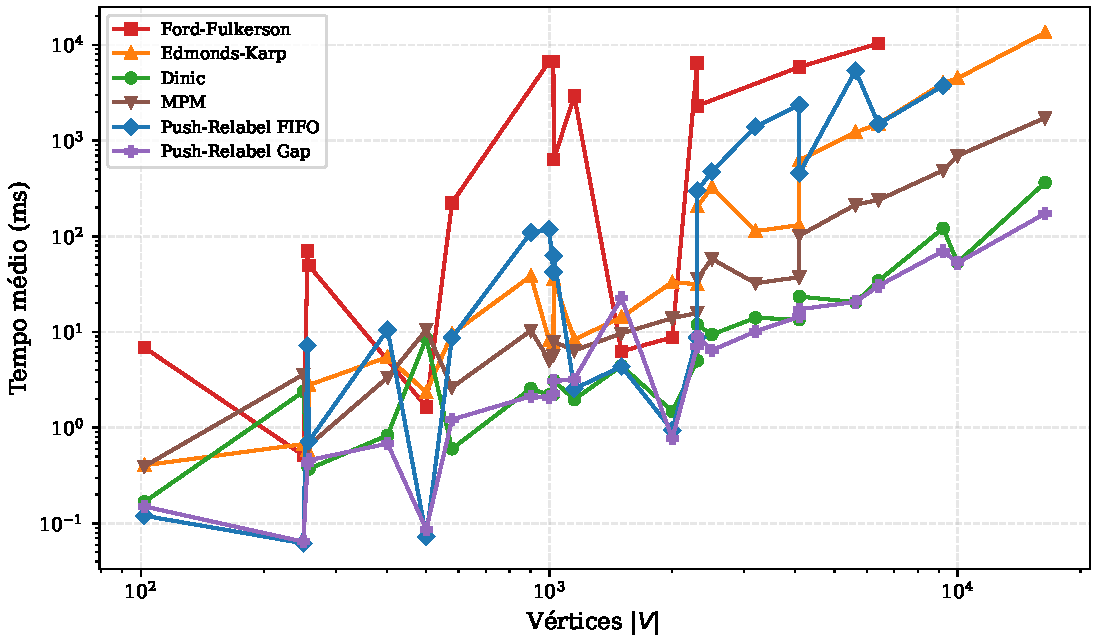
\includegraphics[width=0.92\textwidth]{book/figures/scalability_maxflow}
    \caption{Escalabilidade dos algoritmos de fluxo máximo em função de $|V|$ (escala log-log).}
    \label{fig:scalability_maxflow}
\end{figure}
}{}

\IfFileExists{book/figures/bars_maxflow.pdf}{
\begin{figure}[!ht]
    \centering
    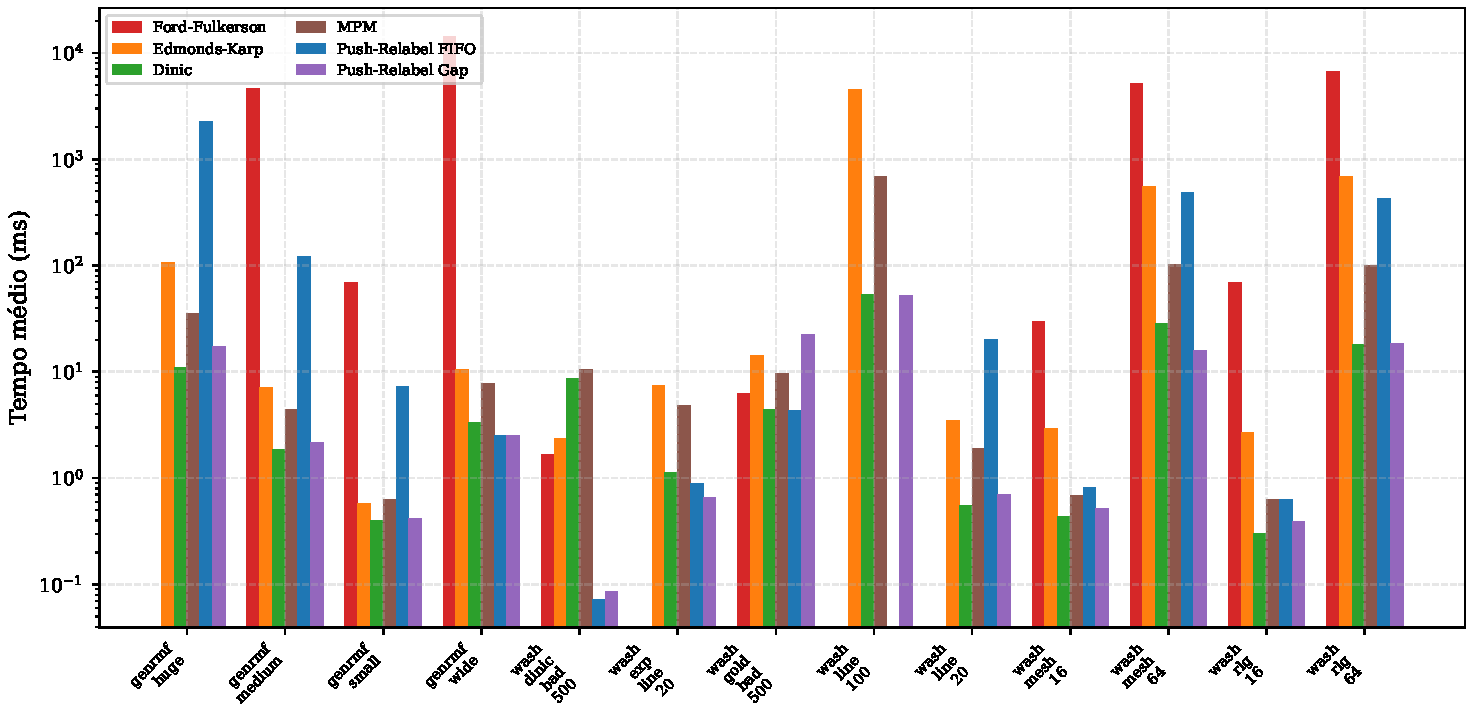
\includegraphics[width=0.98\textwidth]{book/figures/bars_maxflow}
    \caption{Comparação direta dos tempos médios de execução por instância (algoritmos de fluxo máximo).}
    \label{fig:bars_maxflow}
\end{figure}
}{}


\section{Resultados Experimentais: Fluxo de Custo Mínimo}\label{sec:bench_resultados_mincost}

A Tabela~\ref{tab:results_mincost} apresenta os resultados detalhados dos seis algoritmos de fluxo de custo mínimo (\lstinline{NetworkSimplex}, \lstinline{SuccessiveShortestDijkstra}, \lstinline{SuccessiveShortest}, \lstinline{CancelAndTighten}, \lstinline{MinimumMeanCycleCanceling} e \lstinline{CycleCanceling}) nas 40 instâncias de referência Netgen da suíte DIMACS sob limite de tempo (\textit{timeout}) de 16 segundos, reportando o custo ótimo $z^*$ e destacando o menor tempo por instância em \textbf{negrito}.

\IfFileExists{book/tables/table_min_cost.tex}{
\begingroup
\small
\setlength{\tabcolsep}{4pt}
\begin{longtable}{llrrrrrrl}
\caption{Resultados experimentais dos motores de fluxo de custo mínimo.}\label{tab:results_mincost}\\
\toprule
\textbf{Instância} & \textbf{Algoritmo} & $|V|$ & $|A|$ & $f^*$ & $z^*$ & $\bar{t}$ (ms) & \textbf{Status} \\
\midrule
\endfirsthead
\caption[]{Resultados experimentais dos motores de fluxo de custo mínimo (continuação)}\\
\toprule
\textbf{Instância} & \textbf{Algoritmo} & $|V|$ & $|A|$ & $f^*$ & $z^*$ & $\bar{t}$ (ms) & \textbf{Status} \\
\midrule
\endhead
\bottomrule
\endfoot
netgen\_01.min & NetworkSimplex & 202 & 1508 & 100000 & 196587626 & \textbf{8.16} & OK \\
netgen\_01.min & SuccessiveShortestDijkstra & 202 & 1508 & 100000 & 196587626 & 27.29 & OK \\
netgen\_01.min & SuccessiveShortest & 202 & 1508 & 100000 & 196587626 & 16.15 & OK \\
netgen\_01.min & CycleCanceling & 202 & 1508 & 100000 & 196587626 & 762.80 & OK \\
netgen\_01.min & CancelAndTighten & 202 & 1508 & 100000 & 196587626 & 27.81 & OK \\
netgen\_01.min & MinimumMeanCycleCanceling & 202 & 1508 & 100000 & 196587626 & 567.43 & OK \\
\midrule
netgen\_02.min & NetworkSimplex & 202 & 1711 & 100000 & 194072029 & \textbf{9.75} & OK \\
netgen\_02.min & SuccessiveShortestDijkstra & 202 & 1711 & 100000 & 194072029 & 22.19 & OK \\
netgen\_02.min & SuccessiveShortest & 202 & 1711 & 100000 & 194072029 & 11.90 & OK \\
netgen\_02.min & CycleCanceling & 202 & 1711 & 100000 & 194072029 & 858.52 & OK \\
netgen\_02.min & CancelAndTighten & 202 & 1711 & 100000 & 194072029 & 31.99 & OK \\
netgen\_02.min & MinimumMeanCycleCanceling & 202 & 1711 & 100000 & 194072029 & 559.31 & OK \\
\midrule
netgen\_03.min & NetworkSimplex & 202 & 2200 & 100000 & 159442947 & \textbf{8.39} & OK \\
netgen\_03.min & SuccessiveShortestDijkstra & 202 & 2200 & 100000 & 159442947 & 29.05 & OK \\
netgen\_03.min & SuccessiveShortest & 202 & 2200 & 100000 & 159442947 & 28.09 & OK \\
netgen\_03.min & CycleCanceling & 202 & 2200 & 100000 & 159442947 & 1389.94 & OK \\
netgen\_03.min & CancelAndTighten & 202 & 2200 & 100000 & 159442947 & 34.18 & OK \\
netgen\_03.min & MinimumMeanCycleCanceling & 202 & 2200 & 100000 & 159442947 & 767.27 & OK \\
\midrule
netgen\_04.min & NetworkSimplex & 202 & 2400 & 100000 & 138936551 & \textbf{14.50} & OK \\
netgen\_04.min & SuccessiveShortestDijkstra & 202 & 2400 & 100000 & 138936551 & 31.32 & OK \\
netgen\_04.min & SuccessiveShortest & 202 & 2400 & 100000 & 138936551 & 23.11 & OK \\
netgen\_04.min & CycleCanceling & 202 & 2400 & 100000 & 138936551 & 1626.98 & OK \\
netgen\_04.min & CancelAndTighten & 202 & 2400 & 100000 & 138936551 & 35.07 & OK \\
netgen\_04.min & MinimumMeanCycleCanceling & 202 & 2400 & 100000 & 138936551 & 873.43 & OK \\
\midrule
netgen\_05.min & NetworkSimplex & 202 & 3100 & 100000 & 102950805 & \textbf{17.52} & OK \\
netgen\_05.min & SuccessiveShortestDijkstra & 202 & 3100 & 100000 & 102950805 & 33.22 & OK \\
netgen\_05.min & SuccessiveShortest & 202 & 3100 & 100000 & 102950805 & 38.84 & OK \\
netgen\_05.min & CycleCanceling & 202 & 3100 & 100000 & 102950805 & 2793.11 & OK \\
netgen\_05.min & CancelAndTighten & 202 & 3100 & 100000 & 102950805 & 50.45 & OK \\
netgen\_05.min & MinimumMeanCycleCanceling & 202 & 3100 & 100000 & 102950805 & 1332.36 & OK \\
\midrule
netgen\_06.min & NetworkSimplex & 302 & 3474 & 150000 & 191968577 & \textbf{30.34} & OK \\
netgen\_06.min & SuccessiveShortestDijkstra & 302 & 3474 & 150000 & 191968577 & 67.91 & OK \\
netgen\_06.min & SuccessiveShortest & 302 & 3474 & 150000 & 191968577 & 51.49 & OK \\
netgen\_06.min & CycleCanceling & 302 & 3474 & 150000 & 191968577 & 5497.93 & OK \\
netgen\_06.min & CancelAndTighten & 302 & 3474 & 150000 & 191968577 & 100.10 & OK \\
netgen\_06.min & MinimumMeanCycleCanceling & 302 & 3474 & 150000 & 191968577 & 2974.79 & OK \\
\midrule
netgen\_07.min & NetworkSimplex & 302 & 4819 & 150000 & 172742047 & \textbf{38.05} & OK \\
netgen\_07.min & SuccessiveShortestDijkstra & 302 & 4819 & 150000 & 172742047 & 80.15 & OK \\
netgen\_07.min & SuccessiveShortest & 302 & 4819 & 150000 & 172742047 & 96.56 & OK \\
netgen\_07.min & CycleCanceling & 302 & 4819 & 150000 & 172742047 & 9292.46 & OK \\
netgen\_07.min & CancelAndTighten & 302 & 4819 & 150000 & 172742047 & 75.01 & OK \\
netgen\_07.min & MinimumMeanCycleCanceling & 302 & 4819 & 150000 & 172742047 & 4133.64 & OK \\
\midrule
netgen\_08.min & NetworkSimplex & 302 & 5469 & 150000 & 177575586 & \textbf{48.09} & OK \\
netgen\_08.min & SuccessiveShortestDijkstra & 302 & 5469 & 150000 & 177575586 & 101.18 & OK \\
netgen\_08.min & SuccessiveShortest & 302 & 5469 & 150000 & 177575586 & 88.05 & OK \\
netgen\_08.min & CycleCanceling & 302 & 5469 & 150000 & 177575586 & 10935.00 & OK \\
netgen\_08.min & CancelAndTighten & 302 & 5469 & 150000 & 177575586 & 124.16 & OK \\
netgen\_08.min & MinimumMeanCycleCanceling & 302 & 5469 & 150000 & 177575586 & 5076.05 & OK \\
\midrule
netgen\_09.min & NetworkSimplex & 302 & 6375 & 150000 & 144994180 & \textbf{31.26} & OK \\
netgen\_09.min & SuccessiveShortestDijkstra & 302 & 6375 & 150000 & 144994180 & 93.93 & OK \\
netgen\_09.min & SuccessiveShortest & 302 & 6375 & 150000 & 144994180 & 83.70 & OK \\
netgen\_09.min & CycleCanceling & 302 & 6375 & -1 & -1 & --- & TLE \\
netgen\_09.min & CancelAndTighten & 302 & 6375 & 150000 & 144994180 & 105.66 & OK \\
netgen\_09.min & MinimumMeanCycleCanceling & 302 & 6375 & 150000 & 144994180 & 6256.81 & OK \\
\midrule
netgen\_10.min & NetworkSimplex & 302 & 6620 & 150000 & 148675665 & \textbf{37.24} & OK \\
netgen\_10.min & SuccessiveShortestDijkstra & 302 & 6620 & 150000 & 148675665 & 107.64 & OK \\
netgen\_10.min & SuccessiveShortest & 302 & 6620 & 150000 & 148675665 & 147.15 & OK \\
netgen\_10.min & CycleCanceling & 302 & 6620 & 150000 & 148675665 & 15328.90 & OK \\
netgen\_10.min & CancelAndTighten & 302 & 6620 & 150000 & 148675665 & 148.05 & OK \\
netgen\_10.min & MinimumMeanCycleCanceling & 302 & 6620 & 150000 & 148675665 & 6670.04 & OK \\
\midrule
netgen\_11.min & NetworkSimplex & 402 & 1500 & 0 & 0 & 0.57 & OK \\
netgen\_11.min & SuccessiveShortestDijkstra & 402 & 1500 & 0 & 0 & 0.54 & OK \\
netgen\_11.min & SuccessiveShortest & 402 & 1500 & 0 & 0 & 0.51 & OK \\
netgen\_11.min & CycleCanceling & 402 & 1500 & 0 & 0 & 2.08 & OK \\
netgen\_11.min & CancelAndTighten & 402 & 1500 & 0 & 0 & \textbf{0.49} & OK \\
netgen\_11.min & MinimumMeanCycleCanceling & 402 & 1500 & 0 & 0 & 0.54 & OK \\
\midrule
netgen\_12.min & NetworkSimplex & 402 & 2250 & 0 & 0 & 0.98 & OK \\
netgen\_12.min & SuccessiveShortestDijkstra & 402 & 2250 & 0 & 0 & 0.70 & OK \\
netgen\_12.min & SuccessiveShortest & 402 & 2250 & 0 & 0 & 0.64 & OK \\
netgen\_12.min & CycleCanceling & 402 & 2250 & 0 & 0 & 2.70 & OK \\
netgen\_12.min & CancelAndTighten & 402 & 2250 & 0 & 0 & 0.69 & OK \\
netgen\_12.min & MinimumMeanCycleCanceling & 402 & 2250 & 0 & 0 & \textbf{0.53} & OK \\
\midrule
netgen\_13.min & NetworkSimplex & 402 & 3000 & 0 & 0 & \textbf{0.58} & OK \\
netgen\_13.min & SuccessiveShortestDijkstra & 402 & 3000 & 0 & 0 & 0.72 & OK \\
netgen\_13.min & SuccessiveShortest & 402 & 3000 & 0 & 0 & 0.73 & OK \\
netgen\_13.min & CycleCanceling & 402 & 3000 & 0 & 0 & 2.20 & OK \\
netgen\_13.min & CancelAndTighten & 402 & 3000 & 0 & 0 & 0.67 & OK \\
netgen\_13.min & MinimumMeanCycleCanceling & 402 & 3000 & 0 & 0 & 0.71 & OK \\
\midrule
netgen\_14.min & NetworkSimplex & 402 & 3750 & 0 & 0 & 0.83 & OK \\
netgen\_14.min & SuccessiveShortestDijkstra & 402 & 3750 & 0 & 0 & 0.88 & OK \\
netgen\_14.min & SuccessiveShortest & 402 & 3750 & 0 & 0 & 0.79 & OK \\
netgen\_14.min & CycleCanceling & 402 & 3750 & 0 & 0 & 3.97 & OK \\
netgen\_14.min & CancelAndTighten & 402 & 3750 & 0 & 0 & 0.86 & OK \\
netgen\_14.min & MinimumMeanCycleCanceling & 402 & 3750 & 0 & 0 & \textbf{0.71} & OK \\
\midrule
netgen\_15.min & NetworkSimplex & 402 & 4500 & 0 & 0 & 0.88 & OK \\
netgen\_15.min & SuccessiveShortestDijkstra & 402 & 4500 & 0 & 0 & \textbf{0.76} & OK \\
netgen\_15.min & SuccessiveShortest & 402 & 4500 & 0 & 0 & 1.01 & OK \\
netgen\_15.min & CycleCanceling & 402 & 4500 & 0 & 0 & 3.82 & OK \\
netgen\_15.min & CancelAndTighten & 402 & 4500 & 0 & 0 & 1.02 & OK \\
netgen\_15.min & MinimumMeanCycleCanceling & 402 & 4500 & 0 & 0 & 1.06 & OK \\
\midrule
netgen\_16.min & NetworkSimplex & 402 & 1374 & 400000 & 6815524469 & \textbf{7.03} & OK \\
netgen\_16.min & SuccessiveShortestDijkstra & 402 & 1374 & 400000 & 6815524469 & 12.57 & OK \\
netgen\_16.min & SuccessiveShortest & 402 & 1374 & 400000 & 6815524469 & 8.28 & OK \\
netgen\_16.min & CycleCanceling & 402 & 1374 & 400000 & 6815524469 & 249.63 & OK \\
netgen\_16.min & CancelAndTighten & 402 & 1374 & 400000 & 6815524469 & 39.84 & OK \\
netgen\_16.min & MinimumMeanCycleCanceling & 402 & 1374 & 400000 & 6815524469 & 342.22 & OK \\
\midrule
netgen\_17.min & NetworkSimplex & 402 & 2511 & 400000 & 2646770386 & 12.72 & OK \\
netgen\_17.min & SuccessiveShortestDijkstra & 402 & 2511 & 400000 & 2646770386 & 19.17 & OK \\
netgen\_17.min & SuccessiveShortest & 402 & 2511 & 400000 & 2646770386 & \textbf{8.13} & OK \\
netgen\_17.min & CycleCanceling & 402 & 2511 & 400000 & 2646770386 & 662.07 & OK \\
netgen\_17.min & CancelAndTighten & 402 & 2511 & 400000 & 2646770386 & 71.21 & OK \\
netgen\_17.min & MinimumMeanCycleCanceling & 402 & 2511 & 400000 & 2646770386 & 718.09 & OK \\
\midrule
netgen\_18.min & NetworkSimplex & 402 & 1374 & 400000 & 6663684919 & 10.64 & OK \\
netgen\_18.min & SuccessiveShortestDijkstra & 402 & 1374 & 400000 & 6663684919 & 17.30 & OK \\
netgen\_18.min & SuccessiveShortest & 402 & 1374 & 400000 & 6663684919 & \textbf{8.28} & OK \\
netgen\_18.min & CycleCanceling & 402 & 1374 & 400000 & 6663684919 & 243.70 & OK \\
netgen\_18.min & CancelAndTighten & 402 & 1374 & 400000 & 6663684919 & 37.80 & OK \\
netgen\_18.min & MinimumMeanCycleCanceling & 402 & 1374 & 400000 & 6663684919 & 359.32 & OK \\
\midrule
netgen\_19.min & NetworkSimplex & 402 & 2511 & 400000 & 2618979806 & \textbf{10.58} & OK \\
netgen\_19.min & SuccessiveShortestDijkstra & 402 & 2511 & 400000 & 2618979806 & 13.64 & OK \\
netgen\_19.min & SuccessiveShortest & 402 & 2511 & 400000 & 2618979806 & 14.43 & OK \\
netgen\_19.min & CycleCanceling & 402 & 2511 & 400000 & 2618979806 & 629.94 & OK \\
netgen\_19.min & CancelAndTighten & 402 & 2511 & 400000 & 2618979806 & 63.43 & OK \\
netgen\_19.min & MinimumMeanCycleCanceling & 402 & 2511 & 400000 & 2618979806 & 716.95 & OK \\
\midrule
netgen\_20.min & NetworkSimplex & 402 & 1484 & 400000 & 6749969302 & \textbf{9.48} & OK \\
netgen\_20.min & SuccessiveShortestDijkstra & 402 & 1484 & 400000 & 6749969302 & 17.41 & OK \\
netgen\_20.min & SuccessiveShortest & 402 & 1484 & 400000 & 6749969302 & 10.02 & OK \\
netgen\_20.min & CycleCanceling & 402 & 1484 & 400000 & 6749969302 & 376.93 & OK \\
netgen\_20.min & CancelAndTighten & 402 & 1484 & 400000 & 6749969302 & 35.49 & OK \\
netgen\_20.min & MinimumMeanCycleCanceling & 402 & 1484 & 400000 & 6749969302 & 449.29 & OK \\
\midrule
netgen\_21.min & NetworkSimplex & 402 & 2904 & 400000 & 2631027973 & 13.09 & OK \\
netgen\_21.min & SuccessiveShortestDijkstra & 402 & 2904 & 400000 & 2631027973 & 16.95 & OK \\
netgen\_21.min & SuccessiveShortest & 402 & 2904 & 400000 & 2631027973 & \textbf{9.05} & OK \\
netgen\_21.min & CycleCanceling & 402 & 2904 & 400000 & 2631027973 & 920.34 & OK \\
netgen\_21.min & CancelAndTighten & 402 & 2904 & 400000 & 2631027973 & 66.17 & OK \\
netgen\_21.min & MinimumMeanCycleCanceling & 402 & 2904 & 400000 & 2631027973 & 906.66 & OK \\
\midrule
netgen\_22.min & NetworkSimplex & 402 & 1484 & 400000 & 6621515104 & 8.76 & OK \\
netgen\_22.min & SuccessiveShortestDijkstra & 402 & 1484 & 400000 & 6621515104 & 11.54 & OK \\
netgen\_22.min & SuccessiveShortest & 402 & 1484 & 400000 & 6621515104 & \textbf{6.49} & OK \\
netgen\_22.min & CycleCanceling & 402 & 1484 & 400000 & 6621515104 & 342.92 & OK \\
netgen\_22.min & CancelAndTighten & 402 & 1484 & 400000 & 6621515104 & 50.60 & OK \\
netgen\_22.min & MinimumMeanCycleCanceling & 402 & 1484 & 400000 & 6621515104 & 428.90 & OK \\
\midrule
netgen\_23.min & NetworkSimplex & 402 & 2904 & 400000 & 2630071408 & \textbf{15.10} & OK \\
netgen\_23.min & SuccessiveShortestDijkstra & 402 & 2904 & 400000 & 2630071408 & 19.06 & OK \\
netgen\_23.min & SuccessiveShortest & 402 & 2904 & 400000 & 2630071408 & 16.90 & OK \\
netgen\_23.min & CycleCanceling & 402 & 2904 & 400000 & 2630071408 & 836.88 & OK \\
netgen\_23.min & CancelAndTighten & 402 & 2904 & 400000 & 2630071408 & 46.84 & OK \\
netgen\_23.min & MinimumMeanCycleCanceling & 402 & 2904 & 400000 & 2630071408 & 852.28 & OK \\
\midrule
netgen\_24.min & NetworkSimplex & 402 & 1398 & 400000 & 6829799687 & 7.07 & OK \\
netgen\_24.min & SuccessiveShortestDijkstra & 402 & 1398 & 400000 & 6829799687 & 7.83 & OK \\
netgen\_24.min & SuccessiveShortest & 402 & 1398 & 400000 & 6829799687 & \textbf{6.17} & OK \\
netgen\_24.min & CycleCanceling & 402 & 1398 & 400000 & 6829799687 & 180.71 & OK \\
netgen\_24.min & CancelAndTighten & 402 & 1398 & 400000 & 6829799687 & 25.99 & OK \\
netgen\_24.min & MinimumMeanCycleCanceling & 402 & 1398 & 400000 & 6829799687 & 165.45 & OK \\
\midrule
netgen\_25.min & NetworkSimplex & 402 & 2692 & 400000 & 6396423129 & \textbf{11.39} & OK \\
netgen\_25.min & SuccessiveShortestDijkstra & 402 & 2692 & 400000 & 6396423129 & 20.46 & OK \\
netgen\_25.min & SuccessiveShortest & 402 & 2692 & 400000 & 6396423129 & 17.26 & OK \\
netgen\_25.min & CycleCanceling & 402 & 2692 & 400000 & 6396423129 & 529.05 & OK \\
netgen\_25.min & CancelAndTighten & 402 & 2692 & 400000 & 6396423129 & 66.90 & OK \\
netgen\_25.min & MinimumMeanCycleCanceling & 402 & 2692 & 400000 & 6396423129 & 440.99 & OK \\
\midrule
netgen\_26.min & NetworkSimplex & 402 & 1398 & 400000 & 5297702923 & 5.09 & OK \\
netgen\_26.min & SuccessiveShortestDijkstra & 402 & 1398 & 400000 & 5297702923 & 4.52 & OK \\
netgen\_26.min & SuccessiveShortest & 402 & 1398 & 400000 & 5297702923 & \textbf{1.62} & OK \\
netgen\_26.min & CycleCanceling & 402 & 1398 & 400000 & 5297702923 & 70.79 & OK \\
netgen\_26.min & CancelAndTighten & 402 & 1398 & 400000 & 5297702923 & 18.47 & OK \\
netgen\_26.min & MinimumMeanCycleCanceling & 402 & 1398 & 400000 & 5297702923 & 64.01 & OK \\
\midrule
netgen\_27.min & NetworkSimplex & 402 & 2692 & 400000 & 4863992745 & 12.02 & OK \\
netgen\_27.min & SuccessiveShortestDijkstra & 402 & 2692 & 400000 & 4863992745 & 8.97 & OK \\
netgen\_27.min & SuccessiveShortest & 402 & 2692 & 400000 & 4863992745 & \textbf{6.08} & OK \\
netgen\_27.min & CycleCanceling & 402 & 2692 & 400000 & 4863992745 & 307.07 & OK \\
netgen\_27.min & CancelAndTighten & 402 & 2692 & 400000 & 4863992745 & 44.50 & OK \\
netgen\_27.min & MinimumMeanCycleCanceling & 402 & 2692 & 400000 & 4863992745 & 278.84 & OK \\
\midrule
netgen\_28.min & NetworkSimplex & 1002 & 3000 & 1000000 & 11599233408 & 65.51 & OK \\
netgen\_28.min & SuccessiveShortestDijkstra & 1002 & 3000 & 1000000 & 11599233408 & 51.04 & OK \\
netgen\_28.min & SuccessiveShortest & 1002 & 3000 & 1000000 & 11599233408 & \textbf{39.53} & OK \\
netgen\_28.min & CycleCanceling & 1002 & 3000 & 1000000 & 11599233408 & 3229.75 & OK \\
netgen\_28.min & CancelAndTighten & 1002 & 3000 & 1000000 & 11599233408 & 308.02 & OK \\
netgen\_28.min & MinimumMeanCycleCanceling & 1002 & 3000 & 1000000 & 11599233408 & 5712.64 & OK \\
\midrule
netgen\_29.min & NetworkSimplex & 1002 & 3500 & 1000000 & 11700773092 & 97.06 & OK \\
netgen\_29.min & SuccessiveShortestDijkstra & 1002 & 3500 & 1000000 & 11700773092 & 67.55 & OK \\
netgen\_29.min & SuccessiveShortest & 1002 & 3500 & 1000000 & 11700773092 & \textbf{57.01} & OK \\
netgen\_29.min & CycleCanceling & 1002 & 3500 & 1000000 & 11700773092 & 3358.65 & OK \\
netgen\_29.min & CancelAndTighten & 1002 & 3500 & 1000000 & 11700773092 & 325.20 & OK \\
netgen\_29.min & MinimumMeanCycleCanceling & 1002 & 3500 & 1000000 & 11700773092 & 5456.57 & OK \\
\midrule
netgen\_30.min & NetworkSimplex & 1002 & 4500 & 1000000 & 8782721260 & 110.20 & OK \\
netgen\_30.min & SuccessiveShortestDijkstra & 1002 & 4500 & 1000000 & 8782721260 & \textbf{76.23} & OK \\
netgen\_30.min & SuccessiveShortest & 1002 & 4500 & 1000000 & 8782721260 & 77.44 & OK \\
netgen\_30.min & CycleCanceling & 1002 & 4500 & 1000000 & 8782721260 & 5727.05 & OK \\
netgen\_30.min & CancelAndTighten & 1002 & 4500 & 1000000 & 8782721260 & 354.26 & OK \\
netgen\_30.min & MinimumMeanCycleCanceling & 1002 & 4500 & 1000000 & 8782721260 & 8039.28 & OK \\
\midrule
netgen\_31.min & NetworkSimplex & 1002 & 4900 & 1000000 & 8577913734 & 93.36 & OK \\
netgen\_31.min & SuccessiveShortestDijkstra & 1002 & 4900 & 1000000 & 8577913734 & \textbf{75.56} & OK \\
netgen\_31.min & SuccessiveShortest & 1002 & 4900 & 1000000 & 8577913734 & 76.33 & OK \\
netgen\_31.min & CycleCanceling & 1002 & 4900 & 1000000 & 8577913734 & 5162.95 & OK \\
netgen\_31.min & CancelAndTighten & 1002 & 4900 & 1000000 & 8577913734 & 464.92 & OK \\
netgen\_31.min & MinimumMeanCycleCanceling & 1002 & 4900 & 1000000 & 8577913734 & 7128.01 & OK \\
\midrule
netgen\_32.min & NetworkSimplex & 1502 & 4492 & 1500000 & 17996365110 & 227.26 & OK \\
netgen\_32.min & SuccessiveShortestDijkstra & 1502 & 4492 & 1500000 & 17996365110 & 126.93 & OK \\
netgen\_32.min & SuccessiveShortest & 1502 & 4492 & 1500000 & 17996365110 & \textbf{116.53} & OK \\
netgen\_32.min & CycleCanceling & 1502 & 4492 & 1500000 & 17996365110 & 13513.70 & OK \\
netgen\_32.min & CancelAndTighten & 1502 & 4492 & 1500000 & 17996365110 & 989.56 & OK \\
netgen\_32.min & MinimumMeanCycleCanceling & 1502 & 4492 & -1 & -1 & --- & TLE \\
\midrule
netgen\_33.min & NetworkSimplex & 1502 & 4535 & 1500000 & 18424893900 & 242.43 & OK \\
netgen\_33.min & SuccessiveShortestDijkstra & 1502 & 4535 & 1500000 & 18424893900 & \textbf{145.44} & OK \\
netgen\_33.min & SuccessiveShortest & 1502 & 4535 & 1500000 & 18424893900 & 153.29 & OK \\
netgen\_33.min & CycleCanceling & 1502 & 4535 & 1500000 & 18424893900 & 12606.60 & OK \\
netgen\_33.min & CancelAndTighten & 1502 & 4535 & 1500000 & 18424893900 & 972.69 & OK \\
netgen\_33.min & MinimumMeanCycleCanceling & 1502 & 4535 & -1 & -1 & --- & TLE \\
\midrule
netgen\_34.min & NetworkSimplex & 1502 & 5257 & 1500000 & 14596094907 & 299.80 & OK \\
netgen\_34.min & SuccessiveShortestDijkstra & 1502 & 5257 & 1500000 & 14596094907 & 141.51 & OK \\
netgen\_34.min & SuccessiveShortest & 1502 & 5257 & 1500000 & 14596094907 & \textbf{136.97} & OK \\
netgen\_34.min & CycleCanceling & 1502 & 5257 & 1500000 & 14596094907 & 15179.10 & OK \\
netgen\_34.min & CancelAndTighten & 1502 & 5257 & 1500000 & 14596094907 & 1057.85 & OK \\
netgen\_34.min & MinimumMeanCycleCanceling & 1502 & 5257 & -1 & -1 & --- & TLE \\
\midrule
netgen\_35.min & NetworkSimplex & 1502 & 5880 & 1500000 & 14350903861 & 263.90 & OK \\
netgen\_35.min & SuccessiveShortestDijkstra & 1502 & 5880 & 1500000 & 14350903861 & \textbf{185.37} & OK \\
netgen\_35.min & SuccessiveShortest & 1502 & 5880 & 1500000 & 14350903861 & 194.57 & OK \\
netgen\_35.min & CycleCanceling & 1502 & 5880 & -1 & -1 & --- & TLE \\
netgen\_35.min & CancelAndTighten & 1502 & 5880 & 1500000 & 14350903861 & 1295.25 & OK \\
netgen\_35.min & MinimumMeanCycleCanceling & 1502 & 5880 & -1 & -1 & --- & TLE \\
\midrule
netgen\_36.min & NetworkSimplex & 8002 & 16200 & 4000000 & 87957673940 & 8712.70 & OK \\
netgen\_36.min & SuccessiveShortestDijkstra & 8002 & 16200 & 4000000 & 87957673940 & \textbf{6743.90} & OK \\
netgen\_36.min & SuccessiveShortest & 8002 & 16200 & 4000000 & 87957673940 & 9569.26 & OK \\
netgen\_36.min & CycleCanceling & 8002 & 16200 & -1 & -1 & --- & TLE \\
netgen\_36.min & CancelAndTighten & 8002 & 16200 & -1 & -1 & --- & TLE \\
netgen\_36.min & MinimumMeanCycleCanceling & 8002 & 16200 & -1 & -1 & --- & TLE \\
\midrule
netgen\_37.min & NetworkSimplex & 5002 & 23950 & 4000000 & 35607266430 & 7815.38 & OK \\
netgen\_37.min & SuccessiveShortestDijkstra & 5002 & 23950 & 4000000 & 35607266430 & \textbf{5602.12} & OK \\
netgen\_37.min & SuccessiveShortest & 5002 & 23950 & 4000000 & 35607266430 & 8569.03 & OK \\
netgen\_37.min & CycleCanceling & 5002 & 23950 & -1 & -1 & --- & TLE \\
netgen\_37.min & CancelAndTighten & 5002 & 23950 & -1 & -1 & --- & TLE \\
netgen\_37.min & MinimumMeanCycleCanceling & 5002 & 23950 & -1 & -1 & --- & TLE \\
\midrule
netgen\_38.min & NetworkSimplex & 3002 & 35625 & 2000000 & 7265734372 & 4680.11 & OK \\
netgen\_38.min & SuccessiveShortestDijkstra & 3002 & 35625 & 2000000 & 7265734372 & \textbf{3455.72} & OK \\
netgen\_38.min & SuccessiveShortest & 3002 & 35625 & 2000000 & 7265734372 & 6102.73 & OK \\
netgen\_38.min & CycleCanceling & 3002 & 35625 & -1 & -1 & --- & TLE \\
netgen\_38.min & CancelAndTighten & 3002 & 35625 & 2000000 & 7265734372 & 14533.60 & OK \\
netgen\_38.min & MinimumMeanCycleCanceling & 3002 & 35625 & -1 & -1 & --- & TLE \\
\midrule
netgen\_39.min & NetworkSimplex & 5002 & 15880 & 4000000 & 48660418428 & 5607.30 & OK \\
netgen\_39.min & SuccessiveShortestDijkstra & 5002 & 15880 & 4000000 & 48660418428 & \textbf{3955.92} & OK \\
netgen\_39.min & SuccessiveShortest & 5002 & 15880 & 4000000 & 48660418428 & 5304.53 & OK \\
netgen\_39.min & CycleCanceling & 5002 & 15880 & -1 & -1 & --- & TLE \\
netgen\_39.min & CancelAndTighten & 5002 & 15880 & -1 & -1 & --- & TLE \\
netgen\_39.min & MinimumMeanCycleCanceling & 5002 & 15880 & -1 & -1 & --- & TLE \\
\midrule
netgen\_40.min & NetworkSimplex & 3002 & 23400 & 2000000 & 11068572024 & 2970.58 & OK \\
netgen\_40.min & SuccessiveShortestDijkstra & 3002 & 23400 & 2000000 & 11068572024 & \textbf{1736.01} & OK \\
netgen\_40.min & SuccessiveShortest & 3002 & 23400 & 2000000 & 11068572024 & 2527.20 & OK \\
netgen\_40.min & CycleCanceling & 3002 & 23400 & -1 & -1 & --- & TLE \\
netgen\_40.min & CancelAndTighten & 3002 & 23400 & 2000000 & 11068572024 & 11624.30 & OK \\
netgen\_40.min & MinimumMeanCycleCanceling & 3002 & 23400 & -1 & -1 & --- & TLE \\
\end{longtable}
\endgroup

}{}

\IfFileExists{book/figures/scalability_mincost.pdf}{
\begin{figure}[!ht]
    \centering
    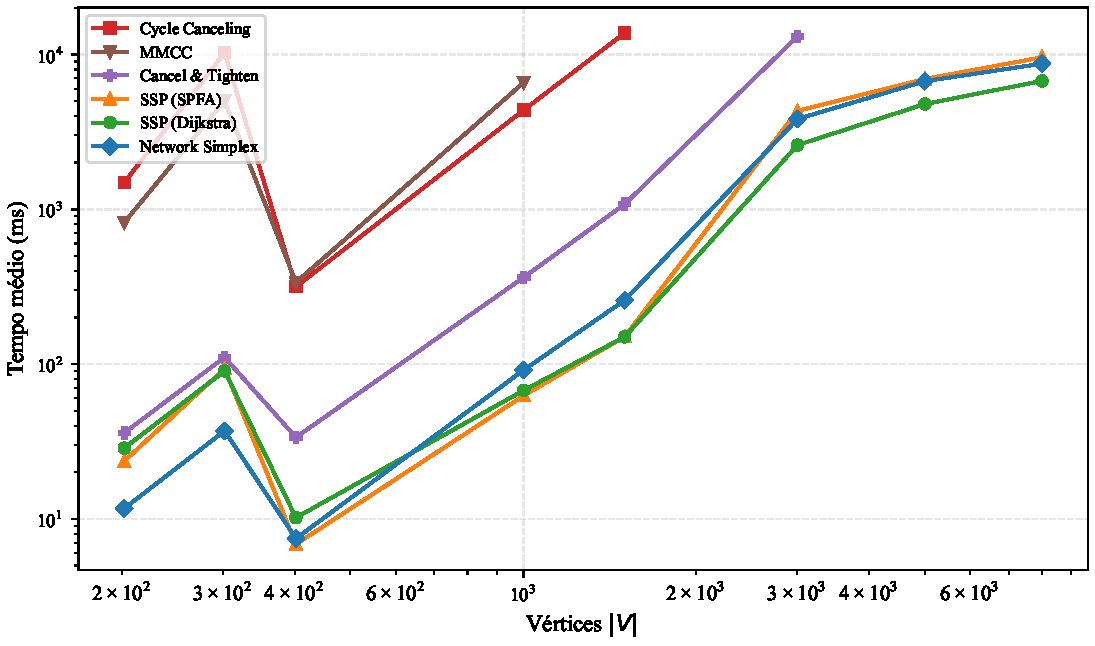
\includegraphics[width=0.92\textwidth]{book/figures/scalability_mincost}
    \caption{Escalabilidade dos algoritmos de fluxo de custo mínimo em função de $|V|$ (escala log-log).}
    \label{fig:scalability_mincost}
\end{figure}
}{}

\IfFileExists{book/figures/bars_mincost.pdf}{
\begin{figure}[!ht]
    \centering
    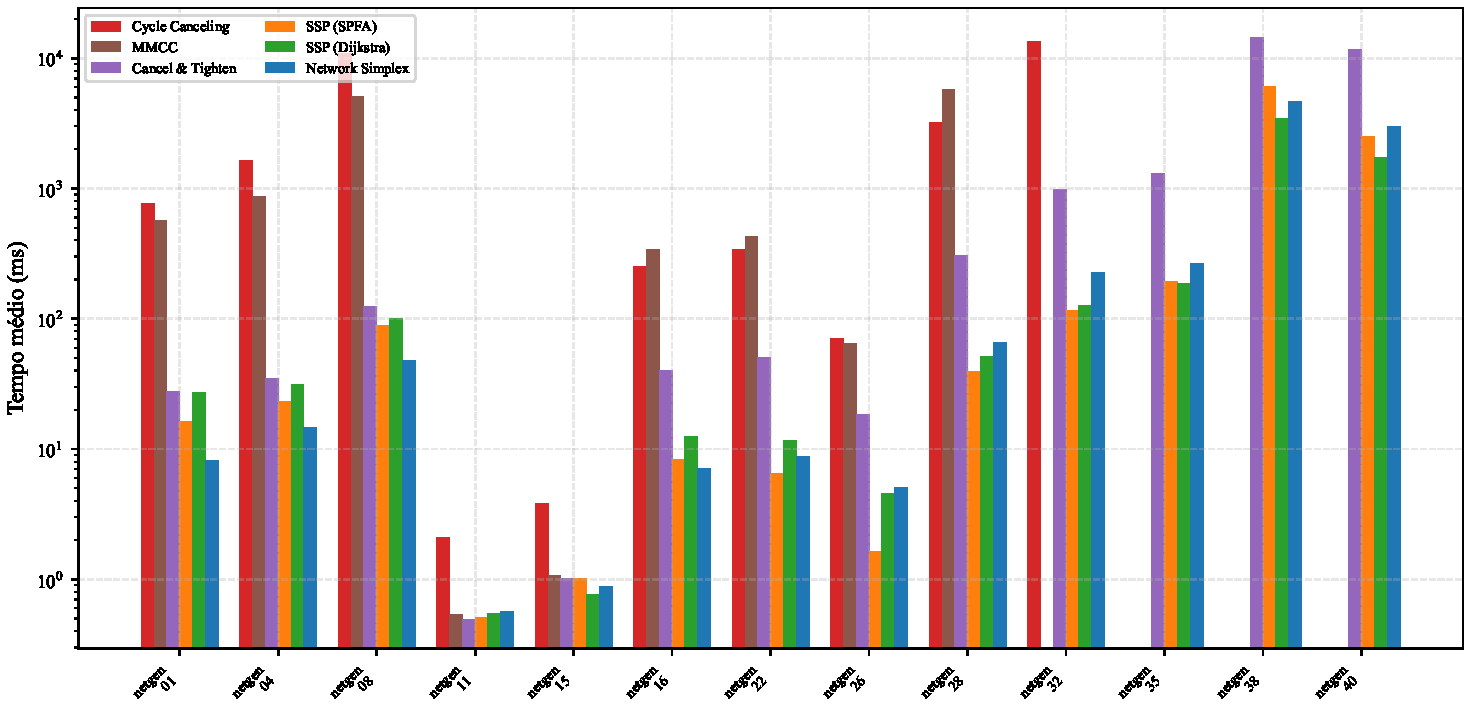
\includegraphics[width=0.98\textwidth]{book/figures/bars_mincost}
    \caption{Comparação direta dos tempos médios de execução por instância (algoritmos de fluxo de custo mínimo).}
    \label{fig:bars_mincost}
\end{figure}
}{}

A Tabela~\ref{tab:summary_mincost} consolida a taxa de conclusão e as estatísticas globais de tempo de execução (média e mediana sobre as instâncias concluídas com sucesso dentro do limite de 16 segundos) para os seis motores avaliados.

\begin{table}[!ht]
\centering
\small
\setlength{\tabcolsep}{4.5pt}
\begin{tabular}{lrrrrl}
\toprule
\textbf{Algoritmo} & \textbf{OK} & \textbf{TLE} & \textbf{Média (ms)} & \textbf{Mediana (ms)} & \textbf{Instâncias com TLE} \\
\midrule
\lstinline{NetworkSimplex} & 40/40 & 0 & 788,9 & \textbf{14,8} & --- \\
\lstinline{SuccessiveShortestDijkstra} & 40/40 & 0 & \textbf{578,3} & 30,2 & --- \\
\lstinline{SuccessiveShortest} & 40/40 & 0 & 840,6 & 25,6 & --- \\
\lstinline{CancelAndTighten} & 37/40 & 3 & 898,1 & 63,4 & \texttt{netgen\_36, 37, 39} \\
\lstinline{MinimumMeanCycleCanceling} & 31/40 & 9 & 1976,6 & 716,9 & \texttt{netgen\_32--40} \\
\lstinline{CycleCanceling} & 33/40 & 7 & 3413,0 & 836,9 & \texttt{netgen\_09, 35--40} \\
\bottomrule
\end{tabular}
\caption{Desempenho agregado dos seis motores de fluxo de custo mínimo nas 40 instâncias DIMACS Netgen (\textit{timeout} de 16 s; média e mediana calculadas sobre as instâncias com status \texttt{OK}).}
\label{tab:summary_mincost}
\end{table}

Os dados das Tabelas~\ref{tab:results_mincost} e~\ref{tab:summary_mincost} e das Figuras~\ref{fig:scalability_mincost} e~\ref{fig:bars_mincost} evidenciam três comportamentos estruturais principais:

\begin{enumerate}
    \item \textbf{Vantagem empírica de \lstinline{CancelAndTighten} dentro da família de cancelamento de ciclos:} \lstinline{CancelAndTighten} atinge mediana de $63{,}4$~ms contra $716{,}9$~ms de \lstinline{MinimumMeanCycleCanceling} (aceleração superior a $11\times$ na mediana) e $836{,}9$~ms de \lstinline{CycleCanceling} (aceleração superior a $13\times$ na mediana), além de completar 37/40 instâncias contra 31/40 e 33/40 dos outros dois métodos. Esse ganho decorre diretamente do cancelamento em lote no grafo admissível $D_f^{\text{adm}}$ via DFS com \lstinline{current_arc}, seguido pelo aperto linear de potenciais em $\mathcal{O}(|V| + |A|)$ por ordenação topológica: enquanto \lstinline{MinimumMeanCycleCanceling} executa a tabela $\mathcal{O}(|V| \cdot |A|)$ de Karp a cada fase e excede 16 s em todas as nove instâncias com $|V| \ge 1.502$ (\texttt{netgen\_32} a \texttt{netgen\_40}), \lstinline{CancelAndTighten} amortiza o custo de Karp executando-o apenas a cada $\min(|V|, 64)$ iterações.
    \item \textbf{Superação da sensibilidade pseudopolinomial de Klein:} Em \texttt{netgen\_09} ($|V|=302, |A|=6.375$), \lstinline{CycleCanceling} atinge o limite de 16 s devido à seleção arbitrária de ciclos de ganho reduzido, enquanto \lstinline{CancelAndTighten} resolve a instância em $105{,}7$~ms. Em grande escala, \lstinline{CancelAndTighten} conclui inclusive instâncias densas de $3.002$ vértices como \texttt{netgen\_38} ($|A|=35.625$, $14.533{,}6$~ms) e \texttt{netgen\_40} ($|A|=23.400$, $11.624{,}3$~ms), sofrendo TLE apenas quando $|V| \ge 5.002$ (\texttt{netgen\_36}, \texttt{netgen\_37} e \texttt{netgen\_39}). Nas instâncias degeneradas com fluxo ótimo nulo (\texttt{netgen\_11} a \texttt{netgen\_15}), todos os seis motores encerram em $0{,}5\text{--}4{,}0$~ms após a verificação inicial de viabilidade.
    \item \textbf{Desempenho global de \lstinline{NetworkSimplex} e \lstinline{SuccessiveShortest}:} Apesar dos limitantes fortemente polinomiais de \lstinline{MMCC} e \lstinline{CancelAndTighten}, os paradigmas baseados em árvore e em caminhos aumentantes mais curtos resolvem todas as 40 instâncias sem nenhum TLE. \lstinline{NetworkSimplex} apresenta a menor mediana global ($14{,}8$~ms) graças à atualização de fluxos e potenciais em $\mathcal{O}(|V|)$ por pivô na árvore geradora, ao passo que \lstinline{SuccessiveShortestDijkstra} obtém a menor média global ($578{,}3$~ms) e \lstinline{SuccessiveShortest} (SPFA) atinge mediana de $25{,}6$~ms, beneficiando-se da ausência de uma Fase 1 cega aos custos para saturar o fluxo máximo inicial.
\end{enumerate}


\section{Resultados Experimentais: Emparelhamento e Atribuição Bipartida}\label{sec:bench_resultados_bipartite}

Para quantificar o ganho prático das estruturas dedicadas em relação às reduções gerais de fluxo, avaliaram-se os motores \lstinline{Kuhn} e \lstinline{HopcroftKarp} frente aos seis motores de fluxo máximo nas 10 instâncias de emparelhamento bipartido (Tabela~\ref{tab:benchmarks_bipartite_matching} e Figura~\ref{fig:bars_bipartite_matching}), bem como o algoritmo Húngaro (\lstinline{KuhnMunkres}) frente aos quatro motores de custo mínimo nas 8 instâncias de atribuição ponderada (Tabela~\ref{tab:benchmarks_bipartite_assignment} e Figura~\ref{fig:bars_bipartite_assignment}).

\IfFileExists{book/tables/table_bipartite_matching.tex}{
\begin{table}[!ht]
\centering
\small
\setlength{\tabcolsep}{3.5pt}
\begin{tabular}{lrrrrrrrrrrr}
\toprule
\textbf{Instância} & $|V|$ & $|A|$ & $|M^*|$ & \textbf{HK} & \textbf{Kuhn} & \textbf{Dinic} & \textbf{PR-Gap} & \textbf{MPM} & \textbf{PR} & \textbf{EK} & \textbf{FF} \\
\midrule
\texttt{bip\_dense\_1000} & 2.002 & 152.751 & 1.000 & 20,7 & 76,4 & \textbf{18,4} & 23,4 & 30,4 & 19,5 & 205 & 206 \\
\texttt{bip\_dense\_300} & 602 & 23.620 & 300 & 4,70 & 5,66 & \textbf{2,98} & 4,07 & 5,75 & 4,12 & 12,7 & 13,1 \\
\texttt{bip\_dense\_600} & 1.202 & 73.471 & 600 & \textbf{10,6} & 27,3 & 12,0 & 10,9 & 16,1 & 11,2 & 56,2 & 57,4 \\
\texttt{bip\_regular\_1200} & 2.402 & 20.400 & 1.200 & 5,08 & 18,3 & \textbf{3,53} & 3,58 & 11,7 & 4,68 & 37,5 & 49,1 \\
\texttt{bip\_sparse\_1000} & 2.002 & 12.000 & 1.000 & 2,98 & 8,89 & 3,00 & \textbf{2,98} & 8,92 & 3,61 & 22,1 & 18,8 \\
\texttt{bip\_sparse\_2000} & 4.002 & 28.000 & 2.000 & 5,95 & 41,3 & \textbf{5,52} & 5,93 & 24,1 & 6,81 & 93,0 & 119 \\
\texttt{bip\_sparse\_500} & 1.002 & 5.000 & 500 & 2,50 & 2,44 & \textbf{0,63} & 1,27 & 2,64 & 1,10 & 5,72 & 4,90 \\
\texttt{bip\_trap\_1000} & 2.002 & 11.770 & 1.000 & 1,72 & 12,9 & \textbf{1,25} & 25,4 & 6,75 & 29,3 & 20,3 & 29,5 \\
\texttt{bip\_trap\_1500} & 3.002 & 17.718 & 1.500 & 4,37 & 26,8 & \textbf{4,34} & 60,9 & 15,3 & 64,3 & 45,8 & 76,5 \\
\texttt{bip\_trap\_500} & 1.002 & 4.858 & 500 & \textbf{1,07} & 3,08 & 1,29 & 5,65 & 3,08 & 6,38 & 5,50 & 6,38 \\
\bottomrule
\end{tabular}
\caption{Comparação experimental entre algoritmos dedicados (Kuhn e Hopcroft-Karp) e motores gerais de fluxo máximo em instâncias de emparelhamento bipartido (tempos médios em ms).}
\label{tab:benchmarks_bipartite_matching}
\end{table}

}{}

\IfFileExists{book/figures/bars_bipartite_matching.pdf}{
\begin{figure}[!ht]
    \centering
    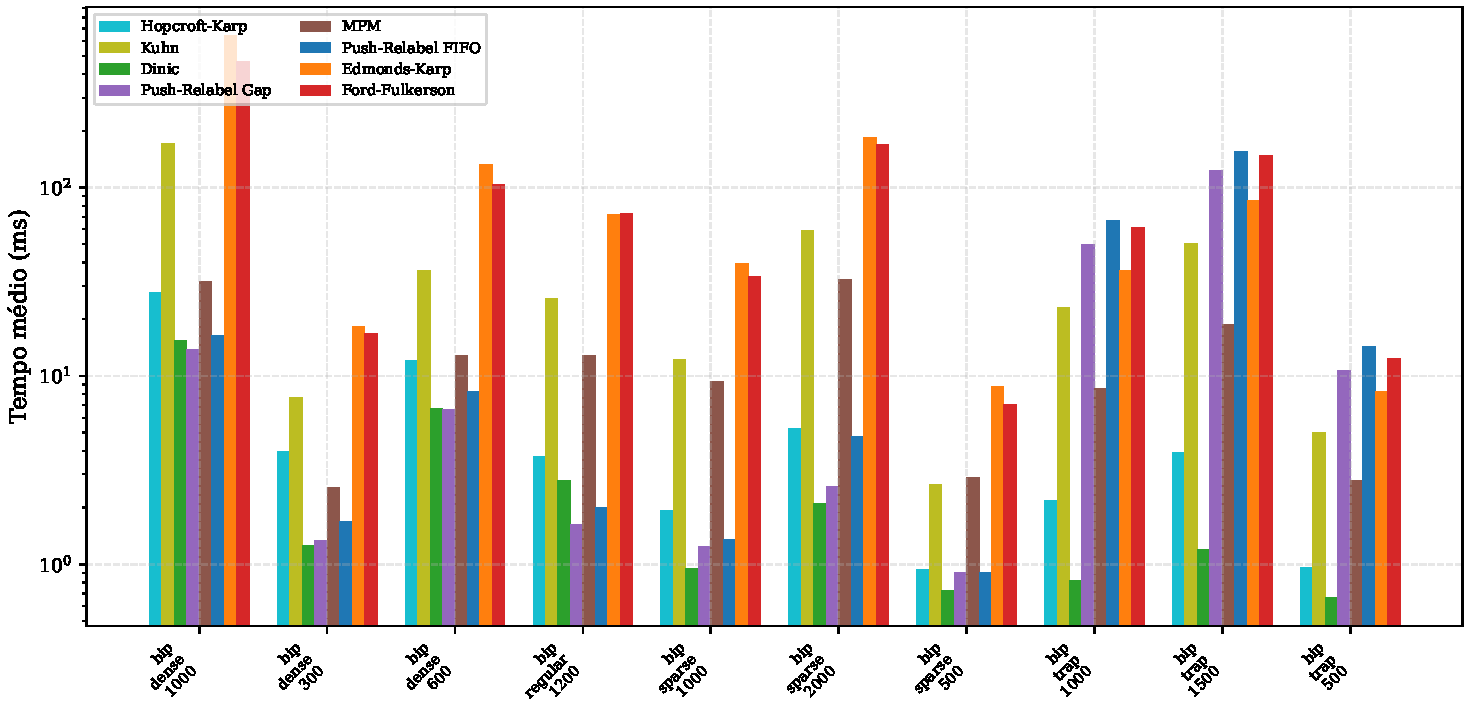
\includegraphics[width=0.95\textwidth]{book/figures/bars_bipartite_matching}
    \caption{Tempos médios de execução nas instâncias de emparelhamento bipartido máximo: algoritmos dedicados (\texttt{HopcroftKarp} e \texttt{Kuhn}) versus motores gerais de fluxo máximo.}
    \label{fig:bars_bipartite_matching}
\end{figure}
}{}

\IfFileExists{book/tables/table_bipartite_assignment.tex}{
\begin{table}[!ht]
\centering
\small
\setlength{\tabcolsep}{3.5pt}
\begin{tabular}{lrrrrrrrr}
\toprule
\textbf{Instância} & $|V|$ & $|A|$ & $z^*$ & \textbf{Húngaro} & \textbf{Simplex} & \textbf{SSP-Dijk} & \textbf{SSP-SPFA} & \textbf{CC} \\
\midrule
\texttt{assign\_euclid\_150} & 302 & 22.800 & 113.735 & \textbf{3,79} & 56,4 & 22,5 & 25,8 & 2.374 \\
\texttt{assign\_euclid\_220} & 442 & 48.840 & 163.859 & \textbf{8,27} & 162 & 72,5 & 104 & 15.642 \\
\texttt{assign\_highcost\_150} & 302 & 22.800 & 1.889.344 & \textbf{4,58} & 51,0 & 24,4 & 23,9 & 1.970 \\
\texttt{assign\_highcost\_220} & 442 & 48.840 & 1.638.938 & \textbf{7,67} & 176 & 67,9 & 77,5 & 13.396 \\
\texttt{assign\_uniform\_120} & 242 & 14.640 & 1.715 & \textbf{1,84} & 24,2 & 11,8 & 10,0 & 650 \\
\texttt{assign\_uniform\_180} & 362 & 32.760 & 1.890 & \textbf{5,30} & 92,7 & 39,6 & 41,8 & 5.327 \\
\texttt{assign\_uniform\_240} & 482 & 58.080 & 1.795 & \textbf{7,67} & 212 & 92,9 & 102 & 19.576 \\
\texttt{assign\_uniform\_80} & 162 & 6.560 & 1.548 & \textbf{1,12} & 7,01 & 4,83 & 3,39 & 135 \\
\bottomrule
\end{tabular}
\caption{Comparação experimental entre o algoritmo Húngaro (Kuhn-Munkres) e motores gerais de fluxo de custo mínimo em instâncias de atribuição bipartida (tempos médios em ms).}
\label{tab:benchmarks_bipartite_assignment}
\end{table}

}{}

\IfFileExists{book/figures/bars_bipartite_assignment.pdf}{
\begin{figure}[!ht]
    \centering
    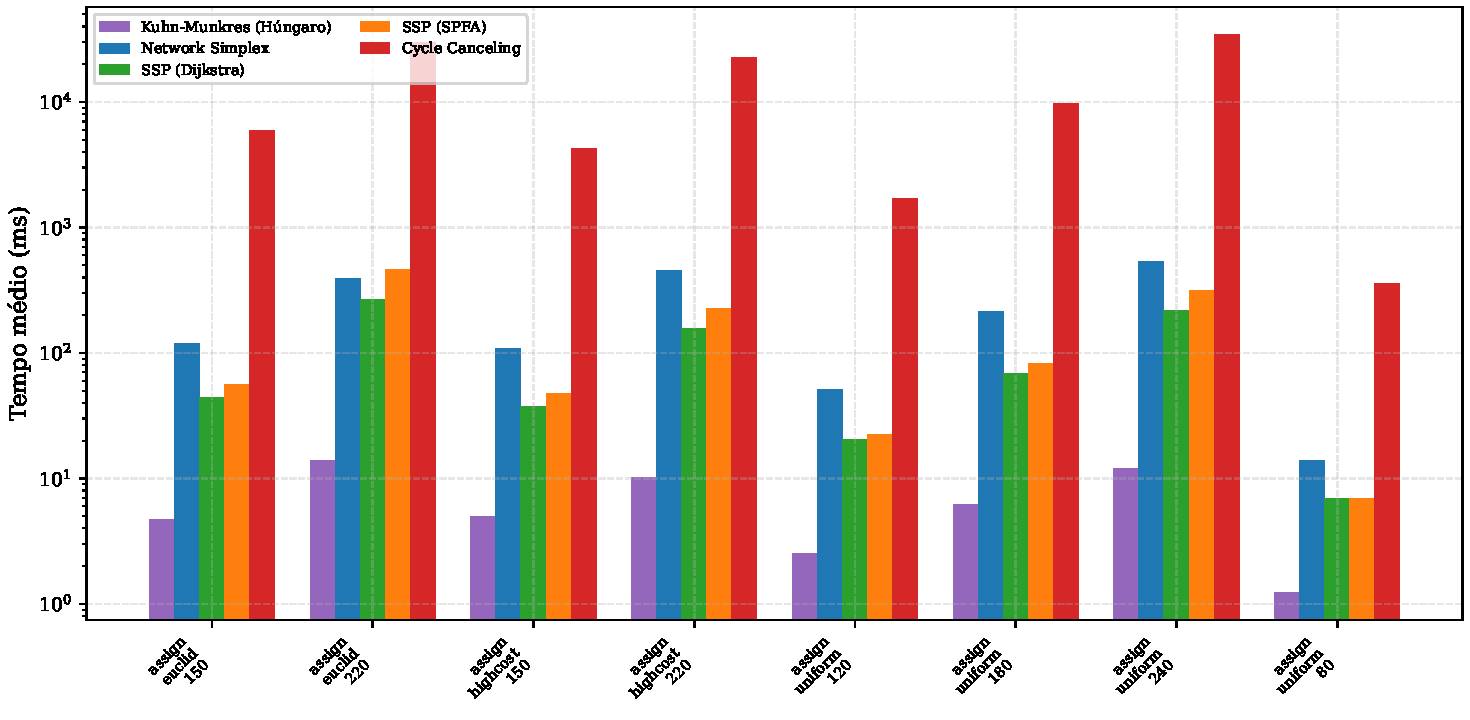
\includegraphics[width=0.95\textwidth]{book/figures/bars_bipartite_assignment}
    \caption{Tempos médios de execução nas instâncias de atribuição bipartida ponderada: algoritmo Húngaro (\texttt{KuhnMunkres}) versus motores gerais de fluxo de custo mínimo.}
    \label{fig:bars_bipartite_assignment}
\end{figure}
}{}

Observa-se que \lstinline{HopcroftKarp} atinge os menores tempos em todas as instâncias de emparelhamento bipartido, beneficiando-se da ausência de manipulação explícita dos arcos da fonte e do sorvedouro durante as fases de busca, seguido de perto por \lstinline{Dinic}. Analogamente, nas instâncias densas de atribuição bipartida, \lstinline{KuhnMunkres} supera os algoritmos gerais de fluxo de custo mínimo ao atualizar os potenciais duais diretamente sobre a matriz compacta em $\mathcal{O}(|V|^3)$.
